%
% FH Technikum Wien
% !TEX encoding = UTF-8 Unicode
%
% Erstellung von Master- und Bachelorarbeiten an der FH Technikum Wien mit Hilfe von LaTeX und der Klasse TWBOOK
%
% Um ein eigenes Dokument zu erstellen, müssen Sie folgendes ergänzen:
% 1) Mit \documentclass[..] einstellen: Master- oder Bachelorarbeit, Studiengang und Sprache
% 2) Mit \newcommand{\FHTWCitationType}.. Zitierstandard festlegen (wird in der Regel vom Studiengang vorgegeben - bitte erfragen)
% 3) Deckblatt, Kurzfassung, etc. ausfüllen
% 4) und die Arbeit schreiben (die verwendeten Literaturquellen in Literatur.bib eintragen)
%
% Getestet mit TeXstudio mit Zeichenkodierung ISO-8859-1 (=ansinew/latin1) und MikTex unter Windows
% Zu beachten ist, dass die Kodierung der Datei mit der Kodierung des paketes inputenc zusammen passt!
% Die Kodierung der Datei twbook.cls MUSS ANSI betragen!
% Bei der Verwendung von UTF8 muss dnicht nur die Kodierung des Dokuments auf UTF8 gestellt sein, sondern auch die des BibTex-Files!
%
% Bugreports und Feedback bitte per E-Mail an latex@technikum-wien.at
%
% Versionen
% *) V0.7: 9.1.2015, RO: Modeline angepasst und verschoben
% *) V0.6: 10.10.2014, RO: Weitere Anpassung an die UK
% *) V0.5: 8.8.2014, WK: Literaturquellen überarbeitet und angepasst
% *) V0.4: 4.8.2014, WK: Initalversion in SVN eingespielt
%
\documentclass[BMR,Bachelor,ngerman]{twbook}%\documentclass[Bachelor,BMR,german]{twbook}
\usepackage[utf8]{inputenc}
\usepackage[T1]{fontenc}
\usepackage{float}
\usepackage{wrapfig}
\usepackage{color}
\usepackage{graphicx,array}
\usepackage{colortbl} 
\usepackage{epic,eepic}
\usepackage{amsgen,amsfonts,amssymb,amsbsy,amsmath,amstext}
\usepackage[official]{eurosym}

%
% Bitte in der folgenden Zeile den Zitierstandard festlegen
\newcommand{\FHTWCitationType}{HARVARD} % IEEE oder HARVARD möglich - wenn Sie zwischen IEEE und HARVARD wechseln, bitte die temorären Dateien (aux, bbl, ...) löschen
%
\ifthenelse{\equal{\FHTWCitationType}{HARVARD}}{\usepackage{harvard}}{\usepackage{bibgerm}}

% Definition Code-Listings Formatierung:
\usepackage[final]{listings}
\lstset{captionpos=b, numberbychapter=false,caption=\lstname,frame=single, numbers=left, stepnumber=1, numbersep=2pt, xleftmargin=15pt, framexleftmargin=15pt, numberstyle=\tiny, tabsize=3, columns=fixed, basicstyle={\fontfamily{pcr}\selectfont\footnotesize}, keywordstyle=\bfseries, commentstyle={\color[gray]{0.33}\itshape}, stringstyle=\color[gray]{0.25}, breaklines, breakatwhitespace, breakautoindent}
\lstloadlanguages{[ANSI]C, C++, [gnu]make, gnuplot, Matlab, Python}

%Formatieren des Quellcodeverzeichnisses
\makeatletter
% Setzen der Bezeichnungen für das Quellcodeverzeichnis/Abkürzungsverzeichnis in Abhängigkeit von der eingestellten Sprache
\providecommand\listacroname{}
\@ifclasswith{twbook}{english}
{%
    \renewcommand\lstlistingname{Code}
    \renewcommand\lstlistlistingname{List of Code}
    \renewcommand\listacroname{List of Abbreviations}
}{%
    \renewcommand\lstlistingname{Quellcode}
    \renewcommand\lstlistlistingname{Quellcodeverzeichnis}
    \renewcommand\listacroname{Abkürzungsverzeichnis}
}
% Wenn die Option listof=entryprefix gewählt wurde, Definition des Entyprefixes für das Quellcodeverzeichnis. Definition des Macros listoflolentryname analog zu listoflofentryname und listoflotentryname der KOMA-Klasse
\@ifclasswith{scrbook}{listof=entryprefix}
{%
    \newcommand\listoflolentryname\lstlistingname
}{%
}
\makeatother
\newcommand{\listofcode}{\phantomsection\lstlistoflistings}

% Die nachfolgenden Pakete stellen sonst nicht benötigte Features zur Verfügung
\usepackage{blindtext}

%
% Einträge für Deckblatt, Kurzfassung, etc.
%
\title{IoT Anwendung für einen Candy Grabber}
\author{Mag.art. Daniela Riedl}
\studentnumber{1510330062}
%\author{Titel Vorname Name, Titel\and{}Titel Vorname Name, Titel}
%\studentnumber{XXXXXXXXXXXXXXX\and{}XXXXXXXXXXXXXXX}
%\supervisor{Richard Otrebski, MSc}
\supervisor[Begutachter]{Richard Otrebski, MSc}
%\supervisor[Begutachterin]{Titel Vorname Name, Titel}
%\secondsupervisor{Titel Vorname Name, Titel}
%\secondsupervisor[Begutachter]{Titel Vorname Name, Titel}
%\secondsupervisor[Begutachterinnen]{Titel Vorname Name, Titel}
\place{Wien}
\kurzfassung{
%Viele Zukunftsvisionen wie Smart Factories und selbstverwaltende Verkehrsnetze basieren auf Dingen, die in der Lage sind, ihre Umgebung wahrzunehmen, die gesammelten Daten zu verarbeiten und diese mit anderen Geräten und Nutzern zu kommunizieren. 
Die Fähigkeit von Dingen zu kommunizieren und ihr Zusammenschluss zu interagierenden Netzwerken wird unter dem Begriff Internet of Things (IoT) zusammengefasst. Täglich werden neue Anwendungsgebiete für das IoT erschlossen und die Anzahl der Dinge im Internet übersteigt bereits die Anzahl der Weltbevölkerung.
%Eine unübersichtliche Anzahl an Softwareplattformen und eingesetzten Kommunikationsprotokollen
Ein wichtiger Katalysator für die Entwicklung von IoT ist die rasche Erstellung von Prototypen um neue Anwendungsfelder zu evaluieren und Ideen auszureifen. Dies gestaltet sich aufgrund der inhärent multidisziplinären Eigenschaften von IoT-Anwendungen und dem derzeitigen Mangel an allgemeinen Architekturstandards als schwierige Aufgabe.
%Eine große Schwierigkeit liegt derzeit in einem Mangel an standardisierten Entwicklungsmethoden und Architekturmodellen für IoT-Anwendungen.
 Um EntwicklerInnen den Einstieg in das IoT zu erleichtern, sind ausgereifte Entwicklungsmethoden zur Prototypen-Erstellung erforderlich.
In dieser Arbeit wurde der Prototyp einer kostengünstigen IoT-Anwendung für einen Spielzeug Candy Grabber entworfen und implementiert. Die Entwicklung des Systems wurde in einem iterativen Prozess mithilfe von Methoden aus dem Prototyping innerhalb eines Monats Entwicklungszeit umgesetzt. Die Auswahl der Toolchain erfolgte in einem fortschreitenden Prozess auf Basis von Recherche und Versuchsaufbauten auf einem Raspberry Pi3.
Als Ergebnis der Experimente wurde eine OPC-Unified Architecture (OPC UA) ausgewählt und mithilfe von \emph{Python OPC-UA} implementiert. Die Benutzerschnittstelle wurde mit Node-RED, einem auf Node-JS basierenden Tool zur Datenflussprogrammierung, verwirklicht. Durch die eingesetzten Prototyping Methoden wie der teilweisen Implementierung kritischer Systemkomponenten während der Planungsphase konnte ein funktionierender Prototyp innerhalb der vorgegebenen Entwicklungszeit erstellt werden.}
%Zu diesem Zweck wurde eine Auswahl von Prototyping-Tools und IoT-Protokollen basierend auf Versuchsaufbauten auf einem Raspberry Pi3 verglichen.
\schlagworte{Internet der Dinge, IoT, Rapid-Prototyping, Node-RED, Raspberry Pi}
\outline{
The smart factories and self managing traffic grids of the future are based on machines and objects that are able to perceive their environment, process the collected data and communicate it with other devices and users. The ability of things to communicate and their integration into intelligent, interacting networks is collectively known as \acf{IOT}. New areas of application for the \ac{IOT} are being opened up on a daily basis and the number of things on the Internet already exceeds the number of the world's population. An important catalyst for the rapid development of \ac{IOT} is the ability to quickly create prototypes to assess the application of new ideas. This is still a complex task, due to the inherently multidisciplinary nature of \ac{IOT} applications. Another difficulty lies in the current lack of standardized development methods and architectural models for \ac{IOT} applications. To help developers get started with the \ac{IOT}, well defined development methods are needed as well as simple and inexpensive prototyping tools. This paper provides an introduction to available development methods and prototyping tools for \ac{IOT} Applications. It describes the solution for modifying and accessing an object to remotely control it via network. To this end, a selection of prototyping tools and \ac{IOT} protocols have been compared and evaluated based on experimental setups on a Raspberry Pi3. As a result to these experiments, an \ac{OPC UA} server-client architecture was chosen and has been implemented with the open license library \emph{Python OPC-UA}. For the client, as well as the graphical user interface, the data flow programming tool Node-RED has been utilized. The use of prototyping methods during the development process, such as experimentation and the partial implementation of critical parts, contributed significantly to the successful creation of a working prototype for remotely controlling a toy candy grabber within one month of development time.}
%To that end, the respective things need to be able to perceive their environment, process the collected data and communicate it with other devices and users. To keep up with the rapidly growing market, simple and inexpensive tools are needed to help developers get started with the \ac{IOT}.   
\keywords{Internet of Things, IoT, Rapid-Prototyping, Node-RED, Raspberry Pi}
\acknowledgements{Bedankung}

\begin{document}

%Festlegungen für den HARVARD-Zitierstandard
\ifthenelse{\equal{\FHTWCitationType}{HARVARD}}{
\bibliographystyle{Harvard_FHTW_MR}%Zitierstandard FH Technikum Wien, Studiengang Mechatronik/Robotik, Version 1.2e
\citationstyle{dcu}%Correct citation-style (Harvardand, ";" between citations, "," between author and year)
\citationmode{abbr}%use "et al." with first citation
\iflanguage{ngerman}{
    %Deutsch Neue Rechtschreibung
    \newcommand{\citepic}[1]{(Quelle: \protect\cite{#1})}%Zitat: Bild
    \newcommand{\citefig}[2]{(Quelle: \protect\cite{#1}, S. #2)}%Zitat: Bild aus Dokument
    \newcommand{\citefigm}[2]{(Quelle: modifiziert "ubernommen aus \protect\cite{#1}, S. #2)}%Zitat: modifiziertes Bild aus Dokument
    \newcommand{\citep}{\citeasnoun}%In-Line Zitiat entweder mit \citep{} oder \citeasnoun{}
    \newcommand{\acessedthrough}{Verf{\"u}gbar unter:}%Für URL-Angabe
    \newcommand{\acessedthroughp}{Verf{\"u}gbar bei:}%Für URL-Angabe (Geschützte Datenbank, Zugriff durch FH)
    \newcommand{\acessedat}{Zugang am}%Für URL-Datum-Angabe
    \newcommand{\singlepage}{S.}%Für Seitenangabe (einzelne Seite)
    \newcommand{\multiplepages}{S.}%Für Seitenangabe (mehrere Seiten)
    \newcommand{\chapternr}{K.}%Für Kapitelangabe
    \renewcommand{\harvardand}{\&}%Harvardand in Zitaten
    \newcommand{\abstractonly}{ausschließlich Abstract}
    \newcommand{\edition}{. Auflage}%Angabe der Auflage
}{
\iflanguage{german}{
    %Deutsch
    \newcommand{\citepic}[1]{(Quelle: \protect\cite{#1})}%Zitat: Bild
    \newcommand{\citefig}[2]{(Quelle: \protect\cite{#1}, S. #2)}%Zitat: Bild aus Dokument
    \newcommand{\citefigm}[2]{(Quelle: modifiziert "ubernommen aus \protect\cite{#1}, S. #2)}%Zitat: modifiziertes Bild aus Dokument
    \newcommand\citet{\citeasnoun}
    \newcommand\citep{\cite}
   % \newcommand{\citet}{\citeasnoun}%In-Line Zitiat entweder mit \citep{} oder \citeasnoun{}
    \newcommand{\acessedthrough}{Verf{\"u}gbar unter:}%Für URL-Angabe
    \newcommand{\acessedthroughp}{Verf{\"u}gbar bei:}%Für URL-Angabe (Geschützte Datenbank, Zugriff durch FH)
    \newcommand{\acessedat}{Zugang am}%Für URL-Datum-Angabe
    \newcommand{\singlepage}{S.}%Für Seitenangabe (einzelne Seite)
    \newcommand{\multiplepages}{S.}%Für Seitenangabe (mehrere Seiten)
    \newcommand{\chapternr}{K.}%Für Kapitelangabe
    \renewcommand{\harvardand}{\&}%Harvardand in Zitaten
    \newcommand{\abstractonly}{ausschließlich Abstract}
    \newcommand{\edition}{. Auflage}%Angabe der Auflage
}}}

\maketitle

%
%
%-------------------------------------------------------------EINLEITUNG
\chapter{Einleitung}
%\acf{IOT}: Kommunikation zwischen Dingen über das Internet.\\ Wichtige Rolle in Cyber physical systems für Industrie 4.0\\ 
Eine Vision für die Industrie der Zukunft ist die Entwicklung intelligenter, vernetzter Fabriken, in denen alle Abläufe vom Bestellvorgang über die Produktion bis hin zur Auslieferung vollautomatisiert ablaufen. Das Produkt selbst wird zu einem kommunizierendem Objekt, dessen Produktionsstatus zu jedem Zeitpunkt abgefragt werden kann. Auch über die Produktionsgrenzen hinaus sollen die Dinge mit anderen Dingen und Nutzern kommunizieren und schließlich zu großflächigen, interagierenden Systemen vernetzt werden. Zusammengefasst werden die kommunizierenden Dinge und deren Vernetzung als \acf{IOT} bezeichnet.\\\newline
% Real world problem: Prototyping im IOT: Interaktive Echtzeitanwendung, kurze Entwicklungszeit, Spatenübergreifende Entwicklungsss
Eine \ac{IOT} Anwendung muss die Kommunikation aller beteiligten Geräte ermöglichen, sollte energieeffizient aufgebaut sein und Sicherheit vor Angriffen von außen gewährleisten. In interaktiven \ac{IOT} Anwendungen und echtzeit-kritischen Cyber-Physischen-Systemen werden geringe Latenzen und eine rasche Reaktionszeit vorausgesetzt. Skalierbarkeit ist ein weiterer wesentlicher Faktor in der Planung von \ac{IOT} Systemen, da die rasch wachsenden Netzwerke die nötigen Kapazitäten für Neuzugänge bereitstellen müssen. Bis 2020 werden laut \citeasnoun{gubbi2013internet} geschätzte 24 Milliarden Dinge das Internet bevölkern. Um mit dem rasant wachsenden Markt mitzuhalten sind einfache und kostengünstige Werkzeuge notwendig um EntwicklerInnen den Einstieg in das \ac{IOT} zu erleichtern. Ein wesentlicher Katalysator für die Entwicklung von \ac{IOT} Anwendungen ist das Erstellen von Prototypen um die Einsatzfelder neuer Ideen zu evaluieren und die Interoperabilität der einzelnen Komponenten eines Systems von Beginn an zu prüfen.\\\newline
%
Rasches Prototyping gestaltet sich aufgrund der inhärent spartenübergreifenden Identität von \ac{IOT} Anwendungen und den oben genannten umfassenden Anforderungen an diese als komplexe Aufgabe. Eine große Schwierigkeit in der Entwicklung von \ac{IOT} Anwendungen ist derzeit laut \citeasnoun{pramudianto2013model} der Mangel an standardisierten Entwicklungsmethoden und Architekturmodellen. Durch die Vielzahl an angebotenen Protokollen und Softwareplattformen wird die Auswahl einer passenden Toolchain noch erschwert.\\\newline
%
Aufgabe dieser Arbeit ist es, den Prototyp einer kostengünstigen \ac{IOT} Anwendung für einen Spielzeug Süssigkeitenautomat (Candy Grabber) zu planen und umzusetzen. Als Grundlage für die Anwendung wird eine Auswahl von Werkzeugen und Protokollen vorgestellt, die im Hinblick auf \ac{IOT} Anwendungen und Rapid Prototyping entwickelt wurden. Anhand von Versuchsaufbauten soll eine Toolchain ausgewählt und durch die Implementierung der Anwendung evaluiert werden.

%Neben den gängigen Internet-Protokollen gibt es Protokolle, die speziell für den Einsatz von Geräten mit geringer Rechenleistung oder für Netzwerke mit niedriger Übertragungsrate entwickelt wurden. Des Weiteren werden Industrieprotokolle in sicherheitsrelevanten Echtzeit-Systemen, sogenannten \emph{Cyber-Physischen Systemen} (Cyber Physical Systems) (CPS) eingesetzt.
%Um mit dem rasant wachsenden Markt mitzuhalten sind einfache und kostengünstige Werkzeuge zur Entwicklung von \ac{IOT} Systemen notwendig um EntwicklerInnen einen raschen Einstieg in das \ac{IOT} zu ermöglichen.
%Forschungsfragen:\\Ausblick auf Thesis
%Die Auswahl der Protokolle zur Umsetzung eines \ac{IOT} Systems ist abhängig von den jeweiligen Systemvoraussetzungen und muss individuell für jedes System angepasst werden. 
%wird durch die Erstellung von Prototyping Versuchsaufbauten mit den vorgestellten Tools getestet und verglichen. Eine \ac{IOT} Anwendung zur Fernsteuerung eines Candy Grabbers soll implementiert werden. Hierfür soll aufbauend auf den vorangegangenen Tests eine passende Toolchain ausgewählt, und diese anhand der Implementierung evaluiert werden. Den unterschiedlichen Strömungen des \ac{IOT} soll hierbei Rechnung getragen werden. Weiters werden Entwicklertools zur Erstellung von \ac{IOT} Prototypen vorgestellt.
\clearpage
%Nachdem das Internet die globale Vernetzung zwischen Personen revolutioniert hat, ist laut \citeasnoun{gubbi2013internet} der nächste Schritt in der Entwicklung des Internets die Interaktion mit realen Objekten und deren Vernetzung zu intelligenten Systemen. Es existiert bereits eine Vielzahl von Anwendungsbereichen für das \ac{IOT} und sie reichen vom privaten und häuslichen Bereich bis hin zu vernetzten Städten. 
%Jeder Anwendungsbereich stellt unterschiedliche Anforderungen an die Entwicklung von \ac{IOT} Anwendungen und birgt andere Herausforderungen. 
%Real world problem:\\%Gesamtherausforderung: viele neue Dinge: Neue Protokolle notwendig, Energieverbrauch effizient gestalten, Sicherheit der IoT systeme gewährleisten, Skalierbarkeit für die schnell wachsenden Netzwerklösungen.
% Real world problem: Prototyping im IOT: Interaktive Echtzeitanwendung, kurze Entwicklungszeit, Spatenübergreifende Entwicklung
%Weiters ist eine effiziente Energieversorgung für mobile Geräte und großflächige Sensor-Netze \acp{WSN} zu gewährleisten um die ökologischen Auswirkungen des \ac{IOT} minimal zu halten. \ac{IOT} Systeme vor Hacker Angriffen und Malware Attacken zu schützen ist besonders im \ac{IIOT} und \ac{CIOT} eine große Herausforderung.
%------------------------------------AUFGABENSTELLUNG
\chapter{Ferngesteuerter Süssigkeitenautomat}
%BILD Candy Grabber
\section{Anforderungen}
Für einen Candy Grabber Süssigkeitenautomat ist eine \ac{IOT} Anwendung zu erstellen. Diese soll die Möglichkeit bieten, den Candy Grabber per Joystick oder per Fernbedienung von einem Computer oder Mobiltelefon zu steuern. Des Weiteren soll es möglich sein, eigene Steuerungsprogramme hochzuladen und zu testen um den Candy Grabber in weiterer Folge als Lernplattform für \ac{IOT} Projekte nutzen zu können.
\begin{figure}[H]
\centering
\includegraphics[width=0.45\linewidth]{./PICs/CandyGrabber.png}
\caption{Fernzusteuernder Candy Grabber}
\end{figure}

\section{Aufgabenstellung}
%\section{Vorgehensweise}
Zur Fernsteuerung des Candy Grabbers müssen Sensordaten sowie Steuersignale erfasst und übertragen werden. Weiters ist es notwendig die Bewegungen des Candy Grabbers beobachten zu können um eine erfolgreiche Steuerung zu ermöglichen. Hierfür sollen die Aufnahmen einer Kamera live über Videostream übertragen werden.
\subsubsection{Hardware}
Die vorhandene Hardware des Candy Grabbers soll möglichst komplett erhalten bleiben um das Budget gering zu halten und die Kompatibilität der Komponenten zu gewährleisten. Zu diesem Zweck wird eine Analyse der Hardware vorgenommen und eine Sensor/Aktorliste erstellt. Des Weiteren soll ein Schaltplan zum Anschluss der Hardware über die Hardware-Schnittstellen (\acp{GPIO}) des ausgewählten \ac{IOT} Geräts erstellt werden. Besonderes Augenmerk ist auf eine gründliche Dokumentation zu legen um die Einarbeitungszeit für nachfolgende Projekte gering zu halten.
\subsubsection{Software}
%Python: He means that Python runs on Windows, Linux, and Mac without issues. C++ would have to be compiled for each OS. Having to compile often makes prototyping slow and less effective.
Die Software soll modular und in einer objektorientierten Programmiersprache implementiert werden. Zur Steuerung des Gerätes soll ein Objekt der Klasse \emph{CandyGrabber} erstellt werden. Dieses Objekt soll den Zugriff auf seine Eigenschaften und Funktionalität über einen Server erlauben und über eine Mensch-Maschinen Schnittstelle (\ac{HMI}) gesteuert werden können. Laut Vorgabe soll dies einerseits über das Bedien-Panel am Gerät und andererseits über eine grafische Oberfläche von der Ferne möglich sein.
%Tabelle Ziele
\begin{table}[H]
\caption{Ziele}
\centering
\begin{tabular}{| p{0.4\textwidth}| p{0.6\textwidth} |}\hline
\rowcolor[gray]{0.9}Ziele & Geplante Umsetzung \\\hline
Funktionalität gewährleisten & Gründliche Analyse der Hardware, Softwaretests, Erstellung von Versuchsaufbauten\\\hline
Gründliche Dokumentation & Erstellung von UML Diagrammen und Schalt- bzw. Kabelplänen sowie Versionierung der Software\\\hline
Modulare Software & Aufteilung des Candy Grabbers in Module, Einsatz von Design Patterns, Hardware Abstraktion \\\hline
Fernsteuerung ermöglichen & Einrichten eines Videostreams, Erstellen einer Webapplikation \\\hline
Eigene Steuerprogramme aufspielbar & Erstellung eines Objekts, Definition von Methoden und Eigenschaften, über Interface zugänglich\\\hline
Präsentation & Erstellung eines Videos, ansprechendes Design der HMI und des Candy Grabber Aufbaus, Spieluntermalung durch das Abspielen von Musikdateien und Tönen\\\hline
%Sicherheit (Security) gewährleisten & Identifikation über Username und Passwort erforderlich\\\hline
\end{tabular}
\end{table}
Besonderes Augenmerk ist auf die Auswahl der Kommunikationsprotokolle und Prototyping Werkzeuge, sowie auf das Design der Systemarchitektur zu legen um die geforderten Eigenschaften einer \ac{IOT} Anwendung umsetzen zu können. Diese Eigenschaften und Grundlegendes zum Aufbau von \ac{IOT} Systemen werden im folgendem Kapitel näher erläutert.
%%Aufgaben
%\begin{table}[!htbp]
%\caption{Vorgehen und Aufgaben}
%\centering
%\begin{tabular}{| p{0.33\linewidth}| p{0.33\linewidth} | p{0.33\linewidth}|}\hline
%\rowcolor[gray]{0.8}Analyse und Planung & &\\\hline
%Auswahl eines \ac{IOT} Geräts & Auswahl zusätzlich benötigter Hardware & Gründliche Dokumentation\\\hline
%Analyse der Original Hardware & Erstellung Sensor/Aktor Liste \newline Entwurf Schaltplan & Anschluss an Rechner\\\hline
%\rowcolor[gray]{0.8}Systementwurf &&\\\hline
%Hardware Abstraktion und Schnittstellen & Systementwurf \newline Klassendiagramm erstellen & Ablauf planen \newline Ablaufdiagramm erstellen\\\hline
%Schnittstellen und Systemgrenzen definieren & Methoden und Properties \newline definieren & Steuerungsprogramm erstellen\\\hline
%\rowcolor[gray]{0.8}Systementwicklung &&\\\hline
%Versuchsaufbauten erstellen & Auswahl der Toolchain &  Aufsetzen eines Servers \\\hline
%Kommunikation mit Client & Webapplikation erstellen & Videostream einrichten\\\hline
%%\rowcolor[gray]{0.8}Systemintegration &&\\\hline


%\end{tabular}
%\end{table}
\clearpage

%------------------------------------------------------------STAND DER TECHNIK
\chapter{Stand der Technik}
%Aufbau Eigenschaften
\ac{IOT} Systeme besitzen nach \citeasnoun{wolf2016architecture} die Fähigkeit Veränderungen bestimmter Parameter durch Sensoren in der physischen Welt wahrzunehmen, die notwendige Rechenleistung um eingehende Datenpakete zu verarbeiten und die Möglichkeit Reaktionen in der physischen Welt durch Aktoren hervorzurufen. Um diese Eigenschaften zu bilden bestehen \ac{IOT} Systeme laut \citeasnoun{gubbi2013internet} aus den drei Grundbausteinen \emph{Hardware}, \emph{Middleware}  und  \emph{Präsentation}. Die \emph{Hardware} dient zur Interaktion mit Objekten und der Umwelt, die \emph{Middleware} ermöglicht die Speicherung und Auswertung von Daten und die \emph{Präsentation} visualisiert und interpretiert die gewonnenen Daten. Wie diese Grundbausteine in einem \ac{IOT} System organisiert werden ist abhängig von der jeweiligen Anwendung. Für die Umsetzung einer \ac{IOT} Anwendung gibt es viele mögliche, vorgeschlagene Architekturmodelle und Visionen.
%-----------------------------------
\section{Architekturmodelle}
In \citeasnoun{wu2010architecture} sind die gängigen \ac{IOT}-Schichtmodelle beschrieben, die bis dato zur Orientierung für \ac{IOT} Architekturen verwendet werden. Das einfachste ist das 3-Ebenen-Modell, bestehend aus einer Wahrnehmungsebene (\emph{Perception layer}), einer Netzwerkebene (\emph{Network-} oder \emph{Transport layer}) und einer Anwendungsebene (\emph{Application layer}).
%
\citeasnoun{wu2010architecture} schlugen eine Erweiterung dieses Modells vor um das Internet der Dinge zu organisieren und kontrollierbar zu gestalten. Aus dem \ac{OSI} Modell und dem \ac{TCP} Modell wurde eine neue \ac{IOT} Architektur abgeleitet und das 3-Ebenen-Modell um eine Bearbeitungsebene (\emph{Processing layer}) und eine Managementebene (\emph{Business layer}) erweitert.
%figure 5 layer
%\begin{figure}[H]
%\centering
%\includegraphics[width=0.35\linewidth]{PICs/5Layers}
%\caption{5-Ebenen-Modell. (Quelle: \protect\citeasnoun{wu2010architecture}, S. 486)}
%\label{5layers}
%\end{figure}
%
%
Mittlerweile existieren zahlreiche Vorschläge von Architekturmodellen für \ac{IOT} Systeme. Unterschiedliche \ac{IOT} Anwendungen erfordern unterschiedliche Schwerpunkte und bisher hat sich noch kein allgemeiner Standard aus den vorgeschlagenen Architekturmodellen herauskristallisiert. Welches Modell zur Systemmodellierung herangezogen wird muss für jede Anwendung gesondert entschieden werden. Abbildung \ref{fig:layer} zeigt einige mögliche \ac{IOT} Architekturmodelle: das 3-Ebenen-Modell, ein Middleware orientiertes Modell, ein auf \ac{SOA} basierendes Modell und eine Variante des 5-Ebenen-Modells von \citeasnoun{wu2010architecture}. Im Folgenden werden die Aufgaben der jeweiligen Schichten näher erläutert.
%Tabelle Aufgaben der Ebenen im IOT
%\begin{table}[H]
%\caption{Aufgaben der Ebenen im \ac{IOT}}
%\label{tab:layers}
%\centering
%\begin{tabular}{| p{0.2\textwidth}| p{0.8\textwidth} |}\hline
%\rowcolor[gray]{0.9}Ebene & Aufgabe \\\hline
\minisec{Perception Layer} Auch \emph{Device Layer} oder \emph{Physical Layer} genannt. Hier werden objektspezifische Sensordaten und Informationen identifiziert und gesammelt. \cite{khan2012future}.
%Daten werden zum Zweck der sicheren Übertragung an den \emph{Transport Layer} weitergeleitet 
\minisec{Transport Layer} Auch \emph{Network Layer} genannt. Dieser gewährleistet die sichere Übertragung der gewonnenen Daten aus dem \emph{Perception Layer} durch ein Übertragungsmedium (kabelgebunden oder kabellos) zum nächsten Layer in dem die Daten verarbeitet werden \cite{khan2012future}.
%
\minisec{Process Layer} Diese Ebene wurde zur Speicherung, Analyse und Verarbeitung der Daten aus dem \emph{Transport Layer} extrahiert.
%
\minisec{Middleware Layer} Auch \emph{Service Management Layer} genannt, ermöglicht es Entwicklern  unterschiedliche Objekte in ihre Anwendungen zu integrieren, ohne die spezifische Hardware-Anbindung jedes Objekts berücksichtigen zu müssen. Dienste (\emph{Services}) können durch die Nutzung von Adressen und Namen an die, die Dienste anfordernden Parteien übermittelt werden. Weiters werden hier wie auch im \emph{Processing Layer} Daten empfangen und verarbeitet \cite{alfuqaha2015survey}.
%
\minisec{Application Layer} Hier findet die Kontextualisierung, Aufbereitung und Visualisierung der Daten statt. Im 3-Ebenen Modell erfüllt der \emph{Application Layer} auch die Aufgaben des \emph{Process Layers}.
%
\minisec{Business Layer} Hier werden die Anwendungen aus dem \emph{Application Layer} organisiert und im Sinne von Langzeitentwicklungen evaluiert. Hierdurch werden Entscheidungsprozesse bezüglich des Einsatzes von Ressourcen und Investments unterstützt.
%\end{tabular}
%\end{table}
%figure other architectures
\begin{figure}[!htbp]
\centering
\includegraphics[width=\textwidth]{PICs/iotArchitecture}
\caption{Die \ac{IOT} Architektur. (a) 3-Ebenen-Modell. (b) Middleware orientiert. (c) SOA basierend. (d) 5-Ebenen-Modell. (Quelle: \protect\cite{alfuqaha2015survey}, S. 2349)}\label{fig:layer}
\end{figure}
%
\par\citeasnoun{ning2011future} schlugen ein weiteres Architekturmodell vor, welches von den menschlichen Fähigkeiten Eindrücke zu verarbeiten, Entscheidungen zu treffen und zu reagieren bzw. agieren inspiriert ist. Dieses besteht aus einem \emph{Gehirn}, dem \emph{Rückenmark} und einem \emph{Nerven-Netzwerk}. Das Gehirn entspricht in diesem Modell der Datenzentrale und ist zuständig für die Datenverarbeitung und das Datenmanagement. Das Rückenmark agiert als verteiltes Netzwerk von Daten-verarbeitenden Knoten und ist für den Transport der Daten zuständig. Ein Netzwerk von Nerven nimmt Veränderungen in der Umgebung wahr und sammelt Informationen, es entspricht also einem Netz aus Sensoren.
%Cloud und Fog Architektur
\section{Systemarchitekturen}
Die meisten \ac{IOT} Systeme sind bisher Cloud-zentriert aufgebaut, das heißt die Daten werden in Cloud Computern gesammelt und verarbeitet. Die Cloud stellt hier die zentrale, verarbeitende Schicht zwischen der darüber liegenden Applikationsschicht und den darunter liegenden vernetzten Objekten dar. Ein weiterer Trend geht derzeit in Richtung einer alternativen Systemarchitektur, dem \emph{Fog Computing}. Hierbei werden die gesammelten Daten bereits in den Sensoren selbst oder in Netzwerks-Zugangsknoten (im boden-nahen Nebel) aufbereitet bevor sie zur weiteren Auswertung in die Cloud gelangen \cite{sethi2017internet}.\\\newline
%Vertikal und Horizontale Architektur
Derzeit werden \ac{IOT} Architekturen weitgehend vertikal integriert und arbeiten unabhängig voneinander. Wenn ein neues Gerät zu einem Netzwerk hinzugefügt werden soll muss dieses vollständig integriert werden, das heißt über alle Schichten hinweg eingebettet werden. \citeasnoun{wolf2016architecture} sehen den Grund für diese vertikale Integrierung in den vielfältigen, individuell angepassten \ac{IOT} Architekturen. Sie schlagen eine horizontal integrierte \ac{IOT} Architektur vor um die Einbindung neuer Objekte zu vereinfachen. \ac{IIOT} Systeme würden allerdings von dieser Architektur nicht profitieren, da in diesen meist die Abgrenzung zu anderen Systemen aus Sicherheitsgründen erfolgen muss und eine individuell angepasste Architektur erwünscht ist.\\\newline
Eine \ac{IOT} Anwendung kann laut \citeasnoun{atzori2010internet} folgenden Paradigmen folgend implementiert werden: internet-orientiert, ding-orientiert oder semantisch-orientiert. Die \ac{IOT} Anwendung muss jedoch immer eine Kreuzung dieser Paradigmen darstellen damit sie laut \citeasnoun{gubbi2013internet} ihre Funktionalität entfalten kann. In diesen unterschiedlichen Visionen sieht \citeasnoun{pramudianto2013model} den Grund für den derzeitigen Mangel an standardisierten Entwicklungsmethoden und Architekturmodellen, der die Entwicklung von \ac{IOT} Anwendungen erschwert.\clearpage
%Im kommerziellen \ac{IOT} wird unterschieden zwischen einem industriellem Internet der Dinge (\ac{IIOT}) und einem gewerblichen Internet der Dinge (\ac{CIOT}) \cite{marcon2017communication}.

%\\\newline\citeasnoun{pramudianto2013model} schlagen eine von der technischen Umsetzung losgelöste, modellgetriebene Entwicklung für \ac{IOT} Anwendungen vor um deren Konzept unabhängig von ihrer konkreten Umsetzung weiterentwickeln zu können.{\color{red} Eventuell zwei Hauptkonzepte herausgreifen und kurz erläutern: IEEE und IETF z.B und Tabelle von Protokollen als Bild einfügen}
%Im \ac{IOT} verschwimmen die Grenzen zwischen Informationstechnologie IT und operativer Technologie (Operational Technology) OT.
%--------------------------------------------------Protokolle
\section{Standards und Protokolle für das \ac{IOT}}
Um die Entwicklung von \ac{IOT} Applikationen voranzutreiben und die Kommunikation zwischen diesen zu fördern arbeiten verschiedene Entwicklerteams an der Standardisierung von Entwicklungsmethoden und Architekturmodellen. Das \ac{W3C}, die \ac{IETF}, das \ac{IEEE} und das \ac{ETSI} erarbeiten Standards für \ac{IOT} Architekturmodelle und Lösungen zu deren Implementierung \cite{alfuqaha2015survey}. Als Standard Protokolle für das \ac{IOT} werden meist das \acf{CoAP} und das \acf{MQTT} Protokoll genannt. Abbildung \ref{fig:protocols} zeigt eine Auswahl der wichtigsten, im \ac{IOT} eingesetzten Kommunikationsprotokolle. Auf die Protokolle \ac{MQTT} und \ac{CoAP} soll in weiterer Folge näher eingegangen werden. Weiters wird das Industrieprotokoll \ac{OPC UA} vorgestellt, welches von der OPC Foundation entwickelt wurde um die plattformunabhängige Interoperabilität von Maschinen zu gewährleisten.
%figure protocols
\begin{figure}[!htbp]
\centering
\includegraphics[width=0.8\textwidth]{PICs/protocols}
\caption{\ac{IOT} Kommunikationsprotokolle auf das \ac{OSI} Modell gemapt (Quelle: \protect\cite{nathali2018iot}, S. 211)}\label{fig:protocols}
\end{figure}
%
%MQTT
\subsection{\acf{MQTT}}
\ac{MQTT} wurde von Andy Stanford-Clark (IBM) und Arlen Nipper (Eurotech) 1999 für die asynchrone Übertragung von Telemetriedaten über unzuverlässige Verbindungen mit schlechter Datenrate entwickelt. Es wurde 2013 als offener Standard von OASIS spezifiziert \cite{mqtt2018specs} und eignet sich speziell für Geräte mit beschränkten Ressourcen und Netzwerke mit niedrigen Datenraten oder unzuverlässiger Datenübertragung \cite{alfuqaha2015survey}. \ac{MQTT} besteht aus einem \emph{Broker}, sowie \emph{Publishern} und \emph{Subscribern}. Daten werden von \emph{Publishern} generiert, unter einem bestimmten \emph{Topic} veröffentlicht und können von Clients die an den Informationen interessiert sind über das jeweilige \emph{Topic} abonniert werden. Der \emph{Broker} informiert die \emph{Subscriber} über Veröffentlichungen in den abonnierten \emph{Topics} und leitet die Daten der \emph{Publisher} weiter. Die zwei wichtigsten Spezifikationen von \ac{MQTT} sind das über \ac{TCP} geroutete MQTT v3.1 sowie MQTT-SN, welches speziell für Sensornetzwerke erstellt wurde und über das \ac{UDP} transportiert wird \cite{alfuqaha2015survey}.
%
%CoAP
\subsection{\acf{CoAP}}
\ac{CoAP} ist ein Übertragungsprotokoll für \ac{IOT} Anwendungen, das von der \ac{IETF} Arbeitsgruppe CoRE (IETF Constrained RESTful Environments) entwickelt wurde und auf dem \ac{REST} Paradigma aufbaut. \ac{REST} ermöglicht es Clients und Servern, Webdienste wie das SOAP (Simple Object Access Protocol) Protokoll zu nutzen. Dabei werden Uni-Form Resource Identifiers (URIs) zur Identifizierung von Ressourcen genutzt und können mittels der \ac{HTTP}-Methoden \emph{get}, \emph{post}, \emph{put} und \emph{delete} abgerufen, veröffentlicht, eingefügt und gelöscht werden \cite{alfuqaha2015survey}. Die eingebundenen \ac{HTTP} Funktionalitäten wurden an \ac{IOT} Geräte mit beschränkten Ressourcen angepasst, daher verbraucht die Kommunikation über \ac{CoAP} laut \citeasnoun{sutaria2013making} 42\% weniger Strom als eine vergleichbare Kommunikation über \ac{HTTP}.
%
%OPC UA
\subsection{\acf{OPC UA}}
%Ursprünglich für die Kommunikation innerhalb eines industriellen Umfelds geplant, eignet sich \ac{OPC UA} aufgrund seiner hohen Skalierbarkeit und Sicherheit auch für den Einsatz in kommerziellen \ac{IOT} Anwendungen. The purpose of the OPC Unified Architecture was to enable a platform-independent interoperability standard for moving data/information between the factory floor and the enterprise. During the course of the development it was obvious that the OPC Unified Architecture was well positioned to expand beyond industrial auto- mation. OPC has expanded into areas of building automation, security, home automation, power generation, packaging, and petrochemicals. Because of the highly scalable architecture of OPC UA, it is also well-positioned for deployment in intelligent embedded devices.
\ac{OPC UA} \cite{opcua} ist ein service-orientiertes Industrie-Protokoll basierend auf einer Client-Server Struktur, welches in der Norm IEC-62541 standardisiert wurde \cite{iec62541}. Die Daten werden objektorientiert modelliert und über den \ac{OPC UA} Server zur Verfügung gestellt. Das \ac{OPC UA} Framework beinhaltet den sogenannten \emph{Adressraum}, indem die Daten als Knoten vorhanden und durch Referenzen miteinander verbunden sind. Clients können diesen Adressraum über Internetdienste durchsuchen (\emph{browsen}) und auf exponierte Daten in diesem zugreifen. Dies kann über das \emph{Binary protocol} oder durch \ac{SOAP} basierende Internetdienste geschehen. Das \emph{Binary Protocol} ist ein Protokoll in Maschinensprache, das bei hohem Datendurchgang eingesetzt wird. \ac{SOAP} Dienste werden hauptsächlich eingesetzt um Probleme mit Firewalls zu umgehen. Der \ac{OPC UA} Standard bietet weiters Authentifizierung und Verschlüsselung in verschiedenen, wählbaren Sicherheitsstufen an \cite{palm2015open}. Aufgrund seiner hohen Skalierbarkeit ist der Einsatz von \ac{OPC UA} auch für \ac{IOT} Anwendungen außerhalb des industriellen Umfelds interessant. Die möglichen Implementierungen von \ac{OPC UA} sind in Abbildung \ref{fig:opcua} zusammengefasst und dem \ac{OSI} Modell gegenübergestellt.
%figure opcua-osi
\clearpage
\begin{figure}[!h]
\centering
\includegraphics[width=0.8\textwidth]{PICs/osi_opcua.png}
\caption{\ac{OPC UA} auf das \ac{OSI} Modell gemapt (Quelle: \protect\cite{neumann2015opcua}, S. 2)}\label{fig:opcua}
\end{figure}
%
%source: http://www.drdobbs.com/web-development/soa-web-services-and-restful-systems/199902676
%\subsection{Service-oriented architecture (SOA)}
%is a paradigm where software components are created with concise interfaces, and each component performs a discrete set of related functions. With its well-defined interface and contract for usage, each component, provides a service to other software components. A web service is an example of an SOA with a well-defined set of implementation choices. In general, the technology choices are SOAP and the Web Service Definition Language (WSDL); both XML-based. WSDL describes the interface (the "contract"), while SOAP describes the data that is transferred. Because of the platform-neutral nature of XML, SOAP, and WSDL, Java is a popular choice for web-service implementation due to its OS-neutrality.
%OPC UA is a protocol for communication in industrial au- tomation, developed by the OPC Foundation and standardized in IEC-62541 [11].
%OPC UA is a protocol for communication in industrial automation, developed by the OPC Foundation and standardized in IEC-62541 [11].
%-------------------------------------------------- Prototyping
\section{Prototyping und Entwicklertools}
Ein Prototyp ist laut \citeasnoun{pomberger1992methoden} \emph{``\dots ein ausführbares Modell mit wesentlichen Eigenschaften des Zielsystems, das Grundlage für die Systemspezifikation ist und die Kommunikation zwischen Kunden und Entwickler unterstützt.''} Zur Erstellung eines Prototypen werden die Schritte Implementierung, Evaluierung und Adaptierung iterativ durchlaufen. Die Entwicklung eines Systems erfolgt nicht in klar voneinander abgetrennten Phasen innerhalb einer sequentiellen Folge sondern besteht aus ineinander übergehenden Phasen die wiederholt durchlaufen werden. Im sogenannten Archtekturprototyping wird ein Prototyp für die Systemarchitektur während der Entwurfsphase erstellt. Dieser bietet die Möglichkeit einer adäquaten Überprüfung des Systems vor der tatsächlichen Implementierung und kann vollständig sein, oder für einzelne, kritische Komponenten und Schnittstellen des Systems erstellt werden. Mithilfe dieser Technik lassen sich Risikos von Fehlentscheidungen sowie Kommunikationsprobleme mit KundInnen während der Spezifikation maßgeblich verringern. Weiters stellt diese Vorgehensweise ein Mittel zur Qualitätssicherung dar und bietet einen hohen Lerneffekt. Die Erstellung von Prototypen ist heutzutage gängige Praxis und kann über den Bau eines realen Produkts oder auch über Umsetzung einer Simulation erfolgen \cite{pomberger1992methoden}.
%\\\newline In the quality gate concept published by the VDMA, the development of a mechatronic system is split up into development stages. At the end of each stage its results are evaluated. The next stage is only commenced if all requirements of the previous stage are met with sufficient quality. Figure 3 depicts the development process of a product and its stages according to the quality gate concept. The three colored lines represent the three basic pillars of a mechatronic system, mechanical engineering, electronic engineering and software engineering (Bender et al., 2006).
%The production line is developed with an iterative approach to ensure compatibility between these disciplines at every stage. Due to this iterative approach structural changes in the template are still possible in the further development process of the production line. Therefore, this thesis documents the current state of development rather than the completed system.\\\newline
%
\\\newline
Um die Entwicklung von \ac{IOT} Prototypen zu vereinfachen existieren eine Auswahl an preiswerten Einplatinencomputern und Entwicklerboards für die Hardwareanbindung sowie eine Vielzahl von Softwareplattformen und Schnittstellen zur Anwendungsprogrammierung (\acp{API}).
\subsection{Entwicklerboards und Einplatinencomputer} 
Für die Realisierung des \emph{Physical Layers} werden für die Erstellung von Prototypen meist Mikrocontroller oder sogenannte Ein-Chip-Systeme (System-on-a-Chip (SoC)) herangezogen. Diese bieten Fähigkeiten zur Datenverarbeitung und Speicherung sowie Schnittstellen zur seriellen Datenübertragung und Netzwerkkommunikation. Mikrocontroller sind SoCs die über einen oder mehrere Prozessorkerne, Arbeitsspeicher (RAM) und nicht flüchtigen Speicher (EPROM) zur Speicherung von Programmen verfügen. Entwicklerboards sind Mikrocontroller, die über zusätzliche Schaltkreise zur einfacheren Programmierung und Hardwareanbindung verfügen. Über \acfp{GPIO} können Sensoren und Aktoren an den Mikrocontroller angeschlossen werden. Des Weiteren werden Datenbusse zur Verfügung gestellt über die eine serielle Kommunikation mit externen Geräten zum Beispiel über \ac{I2C} ermöglicht wird. Ein Beispiel für Entwicklerboards ist die offene Plattform Arduino \cite{arduino2018}. Arduino verfügt über eine große Entwicklergemeinschaft die kompatible Werkzeuge und Entwicklerboards zur Erweiterung des Systems anbieten, zum Beispiel Arduino-UNO oder den Wi-Fi fähigen Mikrocontroller ESP8266-01.\\\newline
Einplatinencomputer (\acp{SBC}) erlauben den Anschluss externer Geräte wie Tastaturen und Bildschirme und bieten eine leistungsstärkere Alternative zu Entwicklerboards. Bekannte Vertreter von Einplatinencomputern sind der Raspberry Pi \cite{rpi2018}, BeagleBone Black \cite{beaglebone2018} oder ODROID \cite{odroid2018}. Viele SBCs entsprechen Miniaturcomputern auf denen ein eingebettetes Betriebssystem läuft. Meistens die gestraffte Variante eines Open Source Linux Betriebssystems. Daher stehen für die Entwicklung von Anwendungen auf SBCs wesentlich mehr Entwicklungstools und Sprachoptionen zur Verfügung als auf Entwicklerboards. Die Kehrseite ist, dass SBCs meist größer, anfälliger für Softwareprobleme und komplexer aufzusetzen sind sowie mehr Energie benötigen. Einplatinencomputer können ähnlich wie Entwicklerboards durch externe Module oder Erweiterungsplatinen, sogenannten HATs im Fall von Raspberry Pi erweitert werden \cite{hardware2018}.
%
\subsection{Softwareplattformen}Oftmals erfordern interaktive \ac{IOT} Anwendungen die Integration von Online-Diensten sowie die Erfassung von Sensordaten und das Auslösen von Reaktionen annähernd in Echtzeit. Um die Entwicklung solcher Systeme zu vereinfachen wurden Tools und Plattformen entwickelt, die die Verknüpfung der einzelnen, datenverarbeitenden Komponenten unterstützen. Diese Plattformen übernehmen Dienste wie Konnektivität und Routing, z.B. \emph{Spacebrew} von \citeasnoun{spacebrew} oder die Verbindung von Services und Dingen über das \emph{Bedingung-Aktion} Paradigma, wie z.B. \emph{zapier} \cite{zapier}. Einige dieser Plattformen bauen auf dem Paradigma der Datenflussprogrammierung auf um die Flexibilität der Programme zu erhöhen und Anwenderfreundlichkeit zu bieten. Ein Beispiel hierfür ist Node-RED \cite{nodered}, ein Open Source Tool zur visuellen Programmierung und Laufzeitumgebung für Datenflussprogramme \cite{giang2014toward}.
\subsection{Node-RED}
%Visual Data Flow Programming Language (VDFPL)
%Node- RED is toolkit for developing data flows on devices and servers.
Node-RED ist ein Web-basiertes Tool zur Vernetzung von \acp{API} und netzwerkfähigen Geräten. Es baut auf dem \emph{Node.js} framework auf, welches eine asynchrone ereignisgesteuerte \emph{JavaScript} Laufzeitumgebung bietet um skalierbare Netzwerkanwendungen zu erstellen \cite{nodejs2018}. Über einen Browser-basierten Flow-Editor können Datenflussprogramme, sogenannte Flows erstellt werden, die auf dem Node-RED Server zur Ausführung bereitgestellt werden. Flows bestehen aus einzelnen Knoten (Nodes), die über Kabel miteinander verbunden sind. Alle Nodes erben von der Node-Basisklasse und sind Unterklassen des \emph{Node.js} \emph{EventEmitters}. Bei der Instanziierung können Nodes externe Dienste abonnieren, auf Daten von einem Port warten oder mit der Verarbeitung von \ac{HTTP}-Anforderungen beginnen. Sobald Daten von einem Node über seinen Eingabe-Handler empfangen wurden, wird die send() Methode der Basisklasse aufgerufen die benannte Ereignisse über die \emph{emit()} Methode des \emph{EventEmitters} an nachgelagerte Nodes sendet. Die nachfolgenden Nodes verarbeiten die Daten, generieren weitere Ereignisse oder kommunizieren mit externen Diensten oder dem Betriebssystem. Es stehen Template-Nodes zu Verfügung, mit denen benutzerdefinierte Nodes erstellt werden können indem eine HTML-Datei hinzugefügt wird, um die Benutzeroberfläche im Browser zu implementieren, sowie eine JavaScript-Datei für die Datenverarbeitung oder Integration auf dem Server. Node-RED ist ein Open Source Projekt, das von IBM und einer großen Gemeinschaft von Benutzern vorangetrieben wird, die Nodes und Flows zum System beisteuern. \cite{giang2014toward}
% %Text representations of flows can be imported and exported between instances. When a node used in one instance of Node-RED is not available on another, a placeholder node is shown in the UI to indicate the user must install a missing node implementation before the flow can be deployed.
%Node-RED’s flows are expressed using JSON as shown in Figure 6. “wires” are not separate objects, but are arrays associated with each node connecting it to a downstream node. Configuration information that may be shared between nodes such as the twitter user name or MQTT topic is held in a configuration node without wires. flows on different tabs or pages are not separated in Node-RED, there is only one flow for the entire system.}
%
%{\color{red}Platform as a Service (PaaS) kostenpflichtige Plattformen}
%PaaS (Platform-as-a-Service) ist eine vollständige Entwicklungs- und Bereitstellungsumgebung in der Cloud, über die Sie Zugang zu den erforderlichen Ressourcen erhalten, um verschiedenste Lösungen bereitstellen zu können – von einfachen cloudbasierten Apps bis hin zu ausgereiften cloudfähigen Unternehmensanwendungen. Sie erwerben die erforderlichen Ressourcen basierend auf einem nutzungsabhängigen Zahlungsmodell von einem Clouddienstanbieter und greifen über eine sichere Internetverbindung darauf zu. {\color{red}https://azure.microsoft.com/de-de/overview/what-is-paas/} PaaS bietet Middleware, Entwicklungstools, BI-Dienste (Business Intelligence), Datenbank-Verwaltungssysteme und mehr. Mit PaaS lässt sich der gesamte Webanwendungs-Lebenszyklus unterstützen – vom Erstellen, Testen und Bereitstellen der Anwendungen bis hin zu deren Verwaltung und Aktualisierung.
%
%\subsection{\acp{API}}
\section{Open Source Projekte}
Open Source Projekte leisten einen wesentlichen Beitrag in der Entwicklung von Prototyping Werkzeugen und Protokollen für das \ac{IOT}. Laut \citeasnoun{palm2015open} können Open Source Projekte als Rückkopplungsschleifen (feedback loops) für Standardisierungsprozesse in der Softwareentwicklung gesehen werden. Weitere Vorteile liegen in der anwenderorientierten und transparenten Entwicklung von Open Source Software und der Möglichkeit, neue Technologien und deren Einsatzgebiete mit geringem finanziellen Risiko auszutesten. \citeasnoun{palm2015open} plädierten für eine Öffnung von Industriestandards um deren Entwicklung in Open Source Projekten voranzutreiben, zum Beispiel für die Erstellung einer Open Source Version von \ac{OPC UA}, die den Ansprüchen eines industriellen Umfelds genügt. %Inzwischen sind mehrere Open Source Implementierungen von \ac{opcua} im Umlauf, inklusive des von \citeasnoun{palm2015open} vorgeschlagenen
%Diese Open Source Version wurde unter dem Namen open62541 \cite{open62541} von der OPC Foundation 
Wichtige Open Source Beiträge zur \ac{IOT} Entwicklung stellen Linux, das Apache HTTP Server Projekt \cite{apache} und das \ac{MQTT} Protokoll dar \cite{mqtt} sowie die verschiedenen Open Source Implementierungen von \ac{OPC UA}, zum Beispiel die C++ Implementierung \emph{open62541} \cite{open62541} oder die Python Implementierung \emph{Python OPC-UA} \cite{pythonopcua2018}.
%\subsection{Raspbian: Linux für Raspberry Pi}
%\subsection{Apache}
%\subsection{RPi web cam Interface}
%\subsection{freeopcua}
%
%https://jaxenter.de/baukasten-fuer-das-internet-dinge-13532
%
%\subsection{REST}
%source: http://www.drdobbs.com/web-development/soa-web-services-and-restful-systems/199902676
%However, there exists an even less restrictive form of SOA than a web service—representational state transfer (REST). Described by Roy Fielding in his doctoral dissertation, REST is a collection of principals that are technology independent, except for the requirement that it be based on HTTP. A system that conforms to the following set of principals is said to be "RESTful":
%All components of the system communicate through interfaces with clearly defined methods and dynamic code.\\
%Each component is uniquely identified through a hypermedia link (URL).\\
%A client/server architecture is followed (web browser and web server).\\
%All communication is stateless.\\
%The architecture is tiered, and data can be cached at any layer.\\
%\\newline Overall, REST can be described as a technology and platform-independent architecture where loosely coupled components communicate via interfaces over standard web protocols. Software, hardware, and data-centric designs maximize system efficiency, scalability, and network throughput. The underlying principal is simplicity.
%Managing and evaluating the applications and provide privacy
%Supporting the decision-making process for the optimal investment and use of new telecommunications resources;
%b) Supporting the management of OA&M related budget;
%c) Supporting the supply and demand of OA&M related manpower; [5J
%d) Maintaining aggregate data about the total enterprise.
%
%\section{Middleware}
%A seemingly obvious solution, maybe from the experience of engineering in the “Internet” world, would be to simply enable the client and the server to be able to handle both the MQTT and CoAP protocols and depending on the remote device capabilities, to send the message in a suitable protocol. But in an environment where the processing and memory availability is highly constrained, implementing multiple protocols on these low- powered devices would not be an ideal situation. Implementing
%multi-protocol libraries and interoperability at the device level should be avoided. Hence, this leads to the need for IOT gateways or middlewares which can provide protocol level interoperability, by translating the data, context or the meaning of the message from one protocol to another protocol. In essence, the IOT gateway should be able to handle a situation where a message comes to a mobile device over the MQTT protocol and the same message, keeping the data (in case of sensing related information) or the command (in case of actuating related instructions) should be translated correctly to the CoAP protocol, without changing the meaning or context of the message.
%\section{Präsentation}
%Daten-Repräsentation und Applicationsdesign, verschiedene Zielsysteme (IOs, Android, Webapplikationen...)
%
\clearpage
%--------------------------------------------------------------KONZEPT & METHODE
\chapter{Angewandte Methoden}
Die Entwicklung des Systems erfolgte in vier Phasen, die nicht strikt sequentiell sondern ineinander übergreifend und teilweise parallel bearbeitet wurden. Diese waren 1. Systemanalyse und Planung, 2. Auswahl der Komponenten durch Versuchsaufbauten, 3. Systementwurf und 4. Implementierung und Systemintegration
%\begin{itemize}
%	\item{Systemanalyse und Planung}
%	\item{Auswahl der Komponenten durch Versuchsaufbauten}
%	\item{Systementwurf}
%	\item{Implementierung}
%\end{itemize}
In den nachfolgenden Abschnitten wird die Vorgehensweise zur Bearbeitung der einzelnen Stufen näher erläutert.
%
\section{Systemanalyse und Planung}
Um die Anforderungen an die Anwendung zu erfassen wurden Analysen der Systemgrenzen sowie der vorhandenen Hardware des Candy Grabbers vorgenommen. Aus diesen wurden die benötigten Ressourcen zur Versorgung des Systems sowie die erforderlichen Hardware-Eigenschaften ermittelt und eine Bestellliste erstellt. %Für die Versorgung der Motoren wurde anhand dieser Daten ein günstiges, einstellbares Netzteil ausgewählt, das bei 3-12V bis zu 600mA liefern kann.

%Analyse der Hardware, Festlegung der Systemgrenzen, Ableitung der benötigten Stromversorgung und Prüfung der möglichen Netzwerkanschlüsse, 
\subsection{Analyse der Hardware}
Zuerst wurde die Funktion des Candy Grabbers getestet und die notwendige Stromversorgung ermittelt. Da der Candy Grabber mit einem Batteriefach für drei Batterien á 1,5V ausgestattet war, wurde das System mit Spannungen von 3,3V bis 5V über ein einstellbares Netzteil versorgt, dabei die Funktion der Motoren beobachtet sowie der Stromverbrauch gemessen. Der Strombedarf bewegte sich dabei bei gleichzeitiger Betätigung von zwei Motoren zwischen 120mA bei 3,3V und 330 mA bei 5V. Alle Sensoren und Aktoren des Geräts waren funktionstüchtig, die Motoren ruckelten jedoch merklich bei einer Spannung unter 4,5V. Anschließend wurde die Platine des Candy Grabbers ausgebaut und mit der Erfassung der Ein- und Ausgänge begonnen. In Abbildung \ref{fig:cgopen} ist das Innenleben des Candy Grabbers abgebildet. Jedem erfassten Aktor und Sensor wurde ein \ac{BMK} nach DIN EN 81346-2 zugeordnet und die Kabel dementsprechend beschriftet. Die Tabellen \ref{tab:Is} und \ref{tab:Os} zeigen eine Auflistung aller Ein- und Ausgänge des Systems sowie deren BMK Nummern.
\begin{figure}[!htbp]
\centering
\includegraphics[width=0.55\textwidth]{PICs/Innenleben_des_candygrabbers_vorher.png}
\caption{Innenleben des Candy Grabbers}\label{fig:cgopen}
\end{figure}
%Tabelle Sensoren/ Aktoren liste
\begin{table}[H]
\centering
%\glqq / \grqq
\caption{Hardware Inputs des Candy Grabbers}\label{tab:Is}
\begin{tabular}{| p{0.08\linewidth} | p{0.27\linewidth} | p{0.4\linewidth} | p{0.15\linewidth} |}\hline
\rowcolor[gray]{0.8} BMK & Bauteil & Beschreibung & Raspberry Pi\\\hline
B1 & Lichtschranke RX & Receiver zeigt Gewinn an & GPIO 27\\
P1 & Lichtschranke TX & Emitterled &  \\\hline
B2 & Referenzschalter & Zeigt Münzeinwurf an & GPIO 16\\\hline
 & Schalter mit 3 Positionen & Zur Motorsteuerung (ON/OFF/ON) &\\
S1 & - & Greifer Links / Rechts & GPIO 24/25 \\
S2 & - & Greifer Vor / Zurück & GPIO 23/22\\
S3 & - & Greifer Hinauf / Hinunter & GPIO 5/6\\\hline
 & Grenztaster & Bei Erreichen einer Endstellung aktiv&\\
B3 & - &  Links & GPIO 18\\
B4 & - &  Rechts & GPIO 17 \\
B5 & - &  Vorne& GPIO 13\\
B6 & - &  Hinten& GPIO 12\\\hline
\end{tabular}
\end{table}
\begin{table}
\caption{Hardware Outputs des Candy Grabbers.}\label{tab:Os}
\begin{tabular}{| p{0.08\linewidth} | p{0.27\linewidth} | p{0.4\linewidth} | p{0.15\linewidth} |}\hline
\rowcolor[gray]{0.8} BMK & Bauteil & Beschreibung & \\\hline
P2 & Lautsprecher & Audioausgabe & Audio Out\\\hline
 & Motoren & Bewegen des Greifers& Motorhat\\
 M1 & - & Links / Rechts & M1\\
 M2 & - & Vor / Zurück & M2\\
 M3 & - & Greifer Hinauf / Hinunter & M3\\\hline
\end{tabular}
\end{table}
%
\subsection{Systemgrenzen}
Der Candy Grabber ist in einem Innenraum stationiert soll aber transportabel bleiben. Es stehen Router für einen Netzwerkanschluss über Ethernet zur Verfügung, die mit dem für Studierende freigegebenen \ac{LAN} der FH Technikum Wien verbunden sind. Im Raum sind mehrere Steckdosen platziert, die eine Stromversorgung über Netzteil ermöglichen. Es müssen keine maßgeblichen Temperaturgrenzen, Einschränkungen des Datenvolumens- oder der Energieversorgung berücksichtigt werden. 
%
\subsection{Materialauswahl}
%Auswahl eines passenden IoT Devices und Erfassung der benötigten Teile für den Einkauf, Erstellung einer Bestellliste. Auswahl des Betriebssystems für das IoT Device und der verwendeten Programmiersprache, Aufsetzen des Geräts.
Nach Analyse der Systemgrenzen wurde die erforderliche Hardware zur Umsetzung des Projekts ausgewählt und bestellt. Die Auswahl erfolgte nach folgenden Kriterien: 
\begin{itemize}
	\item{Tauglichkeit}
	\item{Verfügbarkeit}
	\item{Kosten}
	\item{Qualität der Dokumentation und Simplizität der Anwendung}
\end{itemize}
Weiters wurde ein Betriebssystem sowie eine Programmiersprache für die Implementierung der Anwendung ausgewählt.
\subsubsection{Auswahl des \ac{IOT} Geräts}
Das zum Einsatz kommende \ac{IOT} Gerät muss laut den Anforderungen an ein \ac{IOT} System die Anbindung von Sensoren und Aktoren über Hardware Schnittstellen erlauben, genug Prozessorleistung besitzen um die gewonnenen Daten zu verarbeiten sowie eine Netzwerkanbindung bereitstellen um die gewonnenen Daten zu transportieren. Ein \ac{SBC} bietet sich in diesem Fall zur Umsetzung an, da keine Energie- oder netzwerktechnischen Versorgungsengpässe am Aufstellungsort zu erwarten sind und einige \acp{SBC} über einen Ethernet-Port verfügen.
%
Vor Ort standen ein Odroid-C2 sowie ein Raspberry Pi3 Modell B+ zur Verfügung. Beide verfügen über eine ausreichende Anzahl an \acp{GPIO} und genügend Prozessorleistung sowie einen Netzwerkanschluss. Der C2 von Odroid bietet mehr Rechenleistung und kann mit einer Vollversion des Betriebssystems \emph{Linux Ubuntu} (standardmäßig \emph{Ubuntu  Mate}) oder mit \emph{Android} betrieben werden. Für den  Raspberry Pi3 B+ steht eine Vielzahl von Betriebssystemen zur Verfügung, darunter \emph{Windows 10 IOT}, \emph{Ubuntu Mate} und \emph{RTAndroid}, für die meisten Anwendungen reicht jedoch eine gestraffte Linux Distribution wie zum Beispiel \emph{Raspbian} oder die Raspbian Lite Variante \emph{Noobs} aus. Beide \acp{SBC} befinden sich in derselben Preiskategorie unter \euro{50}. Für die Implementierung wurde der Raspberry Pi3 B+ gewählt da für diesen eine umfassendere Dokumentation existiert und weitreichender Community Support geboten wird.\\\newline
%(https://www.jeffgeerling.com/blog/2016/review-odroid-c2-compared-raspberry-pi-3-and-orange-pi-plus)
%
%Odroid, Raspberry Pi, Arduino. -> RPi gewählt. Überprüfung der Anzahl der benötigten GPIOs und Anschlüsse, sowie Rechenleistung des Geräts. Ausschlaggebender Auswahlgrund: gute Dokumentation zu Raspberry Pi vorhanden. Raspberry Pi: 
Beim Einsatz von \acp{SBC} besteht das Risiko des Datenverlustes, da die verwendeten microSD Karten sehr leicht beschädigt werden können, zum Beispiel durch Temperaturschwankungen. Um dieses Risiko zu minimieren wurden während des weiteren Entwicklungsprozesses regelmäßige Sicherungskopien der SD Karte vorgenommen. Um den Raspberry Pi vor Überhitzung und Staub zu schützen wurde zusätzlich ein Gehäuse und Kühlkörper bestellt.
%
\subsubsection{Auswahl der Programmiersprache und eines Betriebssystem}
Python ist eine objektorientierte Skriptsprache und verfügt laut \citeasnoun{shovic2016raspberry} über den größten Satz an Bibliotheken für \ac{IOT}- und Embedded-System-Geräte für den Raspberry Pi. Des Weiteren ist Python einfach zu lesen und anzuwenden, was diese Programmiersprache für Prototyping attraktiv macht. Python bietet automatisches Speichermanagement und einen interaktiven Modus mit dem kleinere Code-Snippets einfach getestet werden können. Weiters kann man Python um Module erweitern, die in einer kompilierten Sprache wie C oder C++ verfasst wurden. Einer der Nachteile der Anwendung von Python in zeitkritischen Systemen ist, dass die automatische Speicherfreigabe jederzeit eingreifen kann und dabei die Ausführungszeit des laufenden Programms verzögert. Von einer Softwareimplementierung von \ac{PWM} Signalen ist aus diesem Grund abzusehen. Da dies für die Implementierung der Steuerung jedoch kein nennenswertes Hindernis darstellte, wurde Python als Sprache zur Implementierung der Software aus den genannten Gründen ausgewählt. Als Betriebssystem wurde Raspbian Jessie Version 8 gewählt, ein auf Debian Linux basierendes Betriebssystem für den Raspberry Pi. Das neueste Debian Betriebssystem für den Raspberry Pi ist Raspbian Stretch, es wurde jedoch das ältere, stabile Raspbian Jessie bevorzugt da hierzu mehr Dokumentation vorhanden ist.% und da Probleme bei der Installation des \emph{Mosquitto} \ac{MQTT} Servers auf Raspbian Stretch auftreten können.
%issues: of Python is that of the memory garbage collector. Sometimes, your program will run out of memory and Python will invoke the garbage collector to clean up memory and set it up for reuse. This can cause your program to not execute in the time you expected.
%(<< aus Raspberry pi iot projects for makers)
\subsubsection{Motorsteuerung}
Der Greifer des Candy Grabbers wird durch drei DC Motoren bewegt. Die Steuerung der Motoren kann über Vierquadrantensteller (H-Brücke) für den Richtungswechsel und \ac{PWM} für die Geschwindigkeitsregelung realisiert werden.  Die Verwendung eines passenden Erweiterungs-HAT bietet sich hierfür an, da der Raspberry Pi nur über zwei Hardware \ac{PWM} Schnittstellen verfügt. Das \emph{Adafruit DC \& Stepper Motor HAT} \cite{adafruit2018} erlaubt die gleichzeitige Steuerung von vier DC Motoren über einen \ac{PWM} Treiber Chip. Dieser ermöglicht die Regelung der Richtung sowie der Geschwindigkeit mittels \ac{PWM} über die \ac{I2C} Schnittstelle des Raspberry Pi. Für den Anschluss des Motor HAT werden daher nur zwei \ac{GPIO} Pins des Raspberry Pi benötigt. Die Programmierung der Motorsteuerung ist mit der \emph{Adafruit\_MotorHAT} Python Bibliothek sehr einfach umzusetzen, für die Kommunikation über \ac{I2C} muss weiters die \emph{Python smbus} Bibliothek installiert werden sowie die \ac{I2C} Kommunikation in der Configuration des Raspberry Pi aktiviert werden.  Die \ac{GPIO} Pins des Raspberry Pi sind sehr anfällig für Stromspitzen und arbeiten nur sicher in einem Bereich von 2mA-16mA. Daher sollten Motoren und Relais über externe Spannungsquellen versorgt werden. Zum diesem Zweck wurde daher anhand der oben gewonnenen Daten über den Strombedarf des Candy Grabbers ein günstiges, einstellbares Netzteil ausgewählt, das bei 3-12V bis zu 600mA liefern kann. %Das Adafruit MotorHAT bietet hierfür eigene Klemmen für den Anschluss für die Versorgung der Motoren und die interne Motorsteuerung des HAT ist für Spannungen zwischen 5V und 12V ausgelegt.% (https://learn.adafruit.com/adafruit-dc-and-stepper-motor-hat-for-raspberry-pi/powering-motors). 
%
\subsubsection{Kameraauswahl}
Zuletzt wurde eine geeignete Kamera für den Live Video Stream ausgewählt. Die Auswahlkriterien waren ein fixer Fokus um Unschärfen zu vermeiden sowie Kosten und Verfügbarkeit. Die beiden Raspberry Pi Kamera Module v1.3 (5MP) und v.2.1 (8MP) sind mit unter \euro{30} günstiger als Webcams mit vergleichbarer Auflösung und verfügen über einen fixen Fokus. Weiters können diese Module direkt über die \ac{CSI} Schnittstelle am Raspberry Pi angeschlossen werden. Es wurde das ältere Raspberry Pi Kamera Modul v1.3 gewählt, da es günstiger ist und die Auflösung von 5MP bei guter Beleuchtung eine ausreichende Qualität bei geringerem Datenvolumen für den Streaming Dienst bietet. Da das Modul nicht in einem Gehäuse verbaut und anfällig für statische Entladung ist wurde zusätzlich eine Plastikhalterung für die Montage der Kamera an ein Stativ ausgewählt.
\\\newline
Aus der getroffenen Auswahl wurde eine Bestellliste erstellt die in Tabelle \ref{tab:order} ersichtlich ist. Zum Bestellwert kamen noch \euro{11,95} Lieferkosten hinzu. Da der Raspberry Pi bereits zu Verfügung stand beliefen sich die Kosten der Bestellung auf unter \euro{100}.
%Tabelle Bestellliste
\begin{table}[H]
\centering
%\glqq / \grqq
\caption{Bestellliste}
\label{tab:order}
\begin{tabular}{| p{0.1\linewidth} | p{0.7\linewidth} | p{0.1\linewidth} |}\hline
\rowcolor[gray]{0.8} Anzahl & Bezeichnung & Preis\\\hline
	1 & Raspberry Pi3 Modell B+ & \euro{ 36,99}\\\hline
	1 & Raspberry Pi Kamera Modul v1.3 5MP 1080p & \euro{ 20,91}\\\hline
	1 & Flex-Kabel 100cm für Raspberry Pi Kamera Modul & \euro{ 4,20}\\\hline
	1 & Raspberry Pi Kamera Mount & \euro{ 5,00}\\\hline
	1 & Adafruit DC \& Stepper Motor HAT for Raspberry Pi & \euro{ 34,00}\\\hline
	1 & Raspberry Pi Gehäuse & \euro{ 6,00}\\\hline
	1 & Heatsink für Raspberry Pi Aluminium & \euro{ 1,98}\\\hline
	1 & Netzteil für Raspberry Pi (5V/2.5A) &\euro{ 6,00}\\\hline
	1 & Steckernetzteil für DC Motoren einstellbar 3-12V/600mA 7.2W & \euro{ 8,29}\\\hline
	& Summe& \cellcolor[gray]{0.9}\euro{ 123,37}\\\hline
\end{tabular}
\end{table}
%
\section{Auswahl der Komponenten durch Experimente}
Die Auswahl der einzelnen Komponenten erfolgte in einem iterativen Prozess indem die Schritte Implementierung, Evaluierung und Adaptierung zyklisch wiederholt wurden. Es wurden Experimente zur Anbindung der Hardware sowie zur Umsetzung kritischer Schnittstellen des Systems durchgeführt. Die Systemarchitektur wurde mit Hilfe von Architektur Prototyping \cite{pomberger1992methoden} geplant. Dabei wurden kritische Systemteile partiell implementiert um die Kompatibilität und Tauglichkeit der in Frage kommenden \acp{API} und Protokolle zu testen. Die Ergebnisse der durchgeführten Experimente wurden zur Auswahl der Komponenten des Systems herangezogen. Diese wurden nach den Kriterien Kompatibilität der Schnittstellen, Einfachheit der Implementierung, Qualität der Dokumentation und Kosten ausgewählt.
%
\subsection{Hardware-Anbindung und -Schnittstellen}
Auf einem \emph{Breadboard}, einer Steckplatine zur Erstellung von Schaltungs-Prototypen, wurden Experimentier-Schaltungen zum Anschluss der Schalter und Sensoren des Candy Grabbers an den Raspberry Pi aufgebaut und getestet. Die \ac{GPIO} Pins wurden mithilfe des \emph{RPi.GPIO} Python Moduls konfiguriert und ausgelesen. Jeder als Eingang benutzte \ac{GPIO} Pin wurde mit einem \emph{Pull-Up} oder \emph{Pull-Down} Widerstand beschaltet. Diese \emph{ziehen} den Zustand des Pin auf einen standardmäßigen Ausgangswert und schützen ihn vor Beschädigung durch zu hohe Ströme über 16mA. Wird kein Pull-Widerstand eingesetzt springt der Zustand des Pins bei Programmstart undefiniert zwischen High (1) und Low (0) hin und her, was zu einem unerwarteten Verhalten im Programmablauf führen kann. Weiters wurde die Funktion des MotorHATs und die Steuerung der Motoren durch den Anschluss eines 5V DC-Motors an den MotorHAT mit einem erstellten Python-Testprogramm getestet. Hierfür wurde die \emph{Adafruit\_MotorHAT} Library verwendet. \\
%
\par In einem nächsten Schritt wurde der Schalter S1 des Candy Grabbers über die zuvor getestete Schaltung an zwei Pins (links/rechts) des Raspberry Pi angeschlossen um die Richtung des DC Motors mithilfe einer Flankenerkennung zu steuern. \emph{RPi.GPIO} stellt hierfür die Funktion \emph{add\_event\_detect()} zur Verfügung, welcher als Parameter die Nummer des zu überwachenden \ac{GPIO} Pins, die Flankenrichtung des Signals (FALLING für fallend, RISING für steigend oder BOTH für beides) sowie die aufzurufende Rückruffunktion bei einer erkannten Flanke übergeben werden. Der Rückruffunktion kann ein eigener Kanal (channel) als Parameter zugewiesen werden, wodurch ein neuer Thread für die parallele Abarbeitung der Funktion erzeugt wird. Hierdurch wird sichergestellt dass auf jedes \ac{GPIO} Event reagiert wird auch wenn das Hauptprogramm währenddessen mit anderen Prozessen beschäftigt ist. Im folgenden Quellcode \ref{sc:callback} wird eine Veränderung am \ac{GPIO} Eingang 17 erkannt und der Status des Pins über eine Rückruffunktion an der Konsole ausgegeben.\\
%
\begin{lstlisting}[language=Python,name={Beispiel für die Implementierung einer Flankenerkennung am Pin 17 des Raspberry Pi},label={sc:callback}]
	import RPi.GPIO as GPIO	
	# use BCM or BOARD number of pins								
	GPIO.setmode(GPIO.BCM)
	# set up Pin 17 as input and use an internal pull-up resistor							
	GPIO.setup(17, GPIO.IN, pull_up_down=GPIO.PUD_UP)

	# threaded callback function for channel 17
	def callback_function(channel):	
		print(GPIO.input(17))
		
	# add callback for occurring events at GPIO pin 17
	GPIO.add_event_detect(17, GPIO.BOTH, callback=callback_function)
\end{lstlisting}
%
\par Um die Kommunikation mit dem Raspberry Pi über ein Netzwerk zu ermöglichen benötigte das Gerät eine gleichbleibende IP Adresse. Hierfür wurde die Freigabe des Geräts sowie die Vergabe einer statischen IP Adresse für die MAC Adresse des Raspberry Pi im \ac{LAN} der FH Technikum Wien beantragt. Über die zugewiesene IP Adresse kann der Raspberry Pi aus dem gesamten, für Studierende freigegebene \ac{LAN} der FH Technikum Wien erreicht werden.
\begin{table}[H]
\centering
%\glqq / \grqq
\caption{Zugangsdaten des Raspberry Pi}
\label{tab:ipadress}
\begin{tabular}{| p{0.2\linewidth} | p{0.3\linewidth} |}\hline
MAC Adresse & b8:27:eb:c8:a7:51\\\hline
IP Adresse & 10.128.89.61\\\hline
\end{tabular}
\end{table}
%https://sourceforge.net/p/raspberry-gpio-python/wiki/Inputs/
%
%Versuchsaufbauten zur Hardwareanbindung, Aufbau von Schaltungen am Breadboard und RPi Anbindung der Motoren sowie Sensoren. Zuweisung der Ein- und Ausgänge zu passenden, nicht für die I2C Kommunikation des MotorHATs notwendigen GPIOs des Raspberry Pi. Dokumentation.
%
\subsection{Kommunikation} 
Zur Steuerung der Hardware über ein Netzwerk wurden Kommunikationsprotokolle in Versuchsimplementierungen getestet und verglichen um in weiterer Folge eine Auswahl tätigen zu können. Hierfür wurde auf dem Raspberry Pi ein \ac{MQTT} Server sowie ein \ac{OPC UA} Server in Python implementiert. Zum Testen der Kommunikation wurde je ein \emph{Node-RED} Flow erstellt der als Client Anfragen an die testweise implementierten Server stellte. Ein wichtiges Kriterium der Auswahl war daher die vorhandene \emph{Node-RED} Unterstützung des Protokolls. Da die Implementierung der Server ausschließlich mit Open Source Projekten bewerkstelligt wurde waren die Kriterien zur Auswahl die Kompatibilität der Schnittstellen, eine hohe Skalierbarkeit des Protokolls, die Einfachheit der Implementierung und die Qualität der Dokumentation.
%
%\section{Transport und Kommunikation}
%\subsubsection{Node-red Clients}
%Hier wird der Aufbau von Node-RED genauer erläutert. Weiters werden Bilder der Flows der Versuchsaufbauten mit MQTT und OPC UA gezeigt, sowie der Anbindung des Raspberry PIs.
\subsubsection{Node-RED Installation und Anwendung}
Node-RED und das Node.JS Framework sind standardmäßig auf Raspbian Jessie vorinstalliert, sollten aber vor der Verwendung auf die neueste Version aktualisiert werden. Dies wurde durch Eingabe des folgendem Befehls im Terminal des Raspberry Pi erreicht: \begin{verbatim}bash <(curl -sL https://raw.githubusercontent.com/node-red/\ 
raspbian-deb-package/master/resources/update-nodejs-and-nodered)\end{verbatim}
Durch die Eingabe von \verb+node-red-start+ und \verb+node-red-stop+ kann Node-RED gestartet oder gestoppt werden. Über den Befehl \verb+sudo systemctl+ \verb+enable nodered.service+ wird der automatische Start von Node-RED beim Hochfahren des Raspberry Pi aktiviert. Der Flow Editor von Node-RED kann bei laufendem Node-RED Service durch Eingabe der Adresse \verb+http://{ip-adresse-des-raspberry-pi}:1880/+ im Browser aufgerufen werden. Mithilfe des Flow Editors kann man Datenflussprogramme (\emph{Flows}) erstellen indem man vorgefertigte Nodes aus der Palette auf der linken Seite des Node-RED Editors durch \emph{drag \& drop} in den Arbeitsbereich zieht und diese über Kabel (\emph{Wires}) verbindet. Hierfür werden Verbindungslinien von den Outputs der vorgeschalteten Nodes an die Inputs der nachgeschalteten Nodes gezogen. Erstellte Flows kann man durch die \emph{Deploy} Taste im Flow Editor auf den Node-RED Server laden und starten. Unter dem Menüpunkt \emph{Manage palette} können weitere, existierende Nodes installiert und damit zur Palette hinzugefügt werden. In der \emph{Library} können selbst erstellte Nodes und Flows gespeichert werden.
%
\subsubsection{MQTT Server mit \emph{Eclipse Mosquitto}}
Die \ac{MQTT} Kommunikation wird über einen einzelnen, zentralen Server der \emph{Broker} genannt wird abgewickelt. Über sogenannte \emph{Topics} können Nachrichten zwischen Anbietern (\emph{Publisher}) und Abonnenten (\emph{Subscriber}) ausgetauscht werden. Topics sind Bezeichner, über die die Zuordnung der Nachrichten zu einem bestimmten Kanal erfolgt. Für die Testimplementierung wurde der Open Source Broker \emph{Mosquitto} \cite{mosquitto2018} auf dem Raspberry Pi installiert und gestartet. In Node-RED ist standardmäßig der \ac{MQTT} node \emph{mqtt} für die Verbindung mit einen lokalen Broker verfügbar. Dieser kann als Input- oder Output Node konfiguriert werden. Hat man einen mqtt Node im Flow integriert kann man über das \emph{Server Configuration} Pop-Up Menü in einem der mqtt Nodes einen statischen MQTT Config Node durch die Anwahl von \verb+Add an MQTT broker+ erstellen. Standardmäßig wird Port 1883 für die \ac{MQTT} Kommunikation verwendet.\\\newline
Um die Steuerung der Hardware über \ac{MQTT} zu testen wurde der zuvor an den Raspberry Pi angebundene Schalter S1 über zwei \ac{GPIO} Input Nodes eingelesen und damit ein DC Motor über das Topic \emph{/motorOut} gesteuert. Der Node-RED Flow zur Steuerung des Motors über \ac{MQTT} ist in Abbildung \ref{fig:test_mqtt} dargestellt. Der Debug-Node \emph{msg.payload} dient zur Ausgabe der gesendeten Signale im Debug Fenster auf der rechten Seite des Node-RED Flow Editors.
%
\begin{figure}[!htbp]
\centering
\includegraphics[width=0.6\linewidth]{./PICs/mqtt_test.png}
\caption{MQTT Testaufbau in Node-RED}\label{fig:test_mqtt}
\end{figure}
%(https://cookbook.nodered.org/mqtt/connect-to-broker)
%
\subsubsection{OPC UA Server mit Python OPC-UA}
Weiters wurde ein OPC UA Server mit der Open Source Library \emph{Python OPC-UA} \cite{pythonopcua2018} getestet. In Node-RED wurden hierfür zwei mögliche \ac{OPC UA} Implementierungen ausgemacht. \emph{node-red-contrib-opcua} \cite{node-red-opcua} und \emph{node-red-contrib-iiot-opcua} \cite{node-red-iiot-opcua}. Es wurden Versuchsaufbauten mit beiden Implementierungen vorgenommen. Da die Konfigurierung des eigenen \ac{OPC UA} Servers in \emph{node-red-contrib-iiot-opcua} nicht zum erwünschten Verbindungsaufbau des Node-RED Clients mit dem Python OPC UA Server führte konzentrierten sich die weiteren Versuchsaufbauten in Folge auf die ältere Version \emph{node-red-contrib-opcua}. Eine mögliche Ursache für den gescheiterten Verbindungsaufbau könnte sein, dass seitens des OPC UA Config Nodes ein bestimmter Port für den OPC UA Server erwartet wurde, die Dokumentation der \emph{node-red-contrib-iiot-opcua} gab hierzu jedoch keine nähere Auskunft. {\color{purple}Zur Diskussion hinzufügen? Für die Fortsetzung der Experimente und die Umsetzung der Implementierung war die frühere Version \emph{node-red-contrib-opcua} ausreichend, die Umstellung des Flows auf die neuere Version \emph{node-red-contrib-iiot-opcua} wird jedoch empfohlen, da der Support für die frühere Implementierung eingestellt wird.}
%
\\\newline Das Hauptziel des OPC UA Addressraums ist laut \citeasnoun{opcua} Servern die Möglichkeit zu bieten Objekte für Clients standardisiert darzustellen. Das OPC UA Objekt Modell definiert Objekte in Form von Variablen und Methoden. Im Adressraum eines \ac{OPC UA} Servers repräsentiert jedes Objekt einen Knoten, der durch Referenzen mit anderen Knoten verbunden sein kann und dem zur eindeutigen Identifikation eine \emph{NodeId} zugewiesen wird. Die \emph{NodeId} besteht aus den drei Teilen \emph{NamespaceIndex}, \emph{IdentifierType} und \emph{Identifier}. Über die im \ac{OPC UA} \ac{XML} Schema festgelegte \ac{XML} Notation \verb+ns=<NamespaceIndex>;<IdentifierType>=<Identifier>+ kann eine \emph{NodeId} vollständig beschrieben werden. Der \emph{NamespaceIndex} ist ein numerischer Dezimalwert der an Stelle des längeren, für die Identifikation des \emph{Namespace} vergebenen \ac{URI} für Service Anfragen verwendet wird um diese zu optimieren. Die \acp{URI} sind im sogenannten \emph{Namespace array} gespeichert und enthalten die für die Namensgebung der \emph{NodeIds} definierenden Autoritäten wie Normungsgremien und Konsortien (zum Beispiel OPC Foundation), das zugrunde liegende System und den lokalen Server. Der Wert des \emph{NamespaceIndex} eines \emph{Namespace} korrespondiert mit dem Index des zugehörigen \ac{URI} im  \emph{Namespace array}. Der \emph{IdentifierType} beschreibt das Format und den Datentyp des \emph{Identifiers}. Dies kann ein numerischer Wert (i) sein, ein String (s), ein \ac{GUID} (g) oder ein undurchsichtiger, \emph{opaque Value} (b), der ein spezifisches Format des Adressraums als ByteString enthält. Der \emph{Identifier} identifiziert ein bestimmtes Objekt, einen Knoten im Adressraum des \ac{OPC UA} Servers.
Für den Versuchsaufbau wurde der Beispiel Server \emph{example\_server.py} der \emph{Python OPC-UA} Library herangezogen. Auf dem Beispiel-Server ist ein \ac{OPC UA} Objekt angelegt dem die Variablen \emph{myVariable} und \emph{myStringVariable} angehören. In der Testimplementierung sollte der Adressraum des Servers nach bestimmten Variablen durchsucht (BROWSE), die vorhandenen Variablen beschrieben (WRITE) und Änderungen an den Variablen ausgelesen (READ) werden. Hierfür wurden drei Node-RED \ac{OPC UA} Client Nodes (\emph{clientBrowse}, \emph{clientWriteValue} und \emph{subscribeValue}) mit je einer der oben beschriebenen Funktionen (BROWSE, WRITE, READ) erstellt. Abbildung \ref{fig:client_browse} zeigt die Testimplementierung eines Clients mit Browse-Funktion in Node-RED mit \emph{node-red-contrib-opcua}. Im Debug Fenster auf der rechten Seite der Abbildung sieht man die ausgelesenen Informationen über die Variable \emph{MyStringVariable}, zum Beispiel die Beschreibung ihrer \emph{NodeId} mit einem numerischen \emph{Identifier}.  %Objects and their components are represented in the AddressSpace as a set of Nodes described by Attributes and interconnected by References.%http://documentation.unified-automation.com/uasdkhp/1.0.0/html/_l2_ua_node_ids.html
%Diskussion: über Browse sollten die ns am anfang jeder session ausgelesen und an die Client Nodes weitergeleitet werden da sich die ns bei der nächsten Session verändern können.
%In OPC UA service calls the namespace index is used instead of the longer namespace URI in NodeIds. The Client needs to take care of the correct mapping from namespace URI to namespace index. Servers are not allowed to change the namespace index for a specific namespace URI or delete entries from the namespace table as long as an active session exist, so that clients can cache the namespace table for a specific session. But a Server may change namespace indexes and remove entries from the namespace table if no Client is connected or if the server is restarted. For this reason, a Client should not persist the namespace index without storing the namespace URI as well, because a namespace URI represented by index “2” during one session could be represented by index “5” during the next session. Thus, when having established a session with a Server, a Client should always read the Server’s namespace table and update namespace indexes before calling services in which NodeIds are involved.
%
\begin{figure}[H]
\centering
\includegraphics[width=\linewidth]{./PICs/client_browse.png}
\caption{\ac{OPC UA} Testimplementierung von \emph{clientBrowse}}\label{fig:client_browse}
\end{figure}
%
%Auswahl
\par Das Schreiben und Lesen von Variablen war über beide Protokolle umsetzbar. Die Kompatibilität mit den bereits ausgewählten Systemkomponenten war daher bei beiden Protokollen gegeben. Da \ac{OPC UA} speziell zur Interoperabilität von Geräten unterschiedlicher Hersteller entwickelt wurde und es im industriellen Umfeld bereits vielfach angewendet wird, sind die Einsatzmöglichkeiten im Vergleich zu \ac{MQTT} im \ac{IIOT} umfangreicher. Die Umsetzung der Kommunikation über \ac{MQTT} war mit etwas weniger Aufwand verbunden, da ein \ac{MQTT} Node standardmäßig in der Palette von Node-RED vorhanden ist. Des Weiteren existieren zahlreiche Beispiel-Implementierungen für den \emph{Mosquitto} Broker auf dem Raspberry Pi. Für die Implementierung von \emph{Python OPC-UA} existieren ebenfalls gut kommentierte Beispiel-Implementierungen \cite{pythonopcua2018} sowie eine Online-Dokumentation \cite{doku2015pyopcua}. Das Aufbauen des Adressraumes über \ac{XML} kann beim Starten des \ac{OPC UA} Servers auf leistungsschwächeren Geräten wie dem Raspberry Pi sehr viel Zeit in Anspruch nehmen. Diese Zeit kann laut \citeasnoun{pythonopcua2018} verringert werden indem man im Konstruktor des Servers den Pfad zu einer Cache-Datei hinterlegt. Der erste Startvorgang dauert hiermit wesentlich länger, danach reduziert sich die Dauer des Startvorgangs bei einer zuvor benötigten Zeit von beispielsweise 125sec auf ungefähr 3,5sec bei nachfolgenden Startvorgängen auf einem Raspberry Pi3 Modell B \cite{pythonopcua2018}. Abgesehen von der Dauer des Startvorgangs wurde die Kommunikation beider Protokolle über Node-RED als ausreichend flüssig für die Implementierung der Steuerung erachtet. Es wurde das \ac{OPC UA} Protokoll aufgrund seiner sehr hohen Skalierbarkeit, wählbaren Sicherheitsstufen und der standardisierten Darstellung von Objekten für die Implementierung ausgewählt.
%Auswahl: OPC UA setzt objektorientierte Modellierung voraus, ist kompatibel mit industriellen Umgebungen, hat integrierte security die anpassbar ist (in mehreren Sicherheitsstufen). MQTT hat weniger overhead, ist aber für diese Anwendung nicht so kritisch wegen Anschluss ans LAN. Beides hat funktioniert, opc ua wurde ausgewählt.
\subsection{Kamera Live-Übertragung}
Um die Fernsteuerung des Candy Grabbers zu ermöglichen wurde die Live-Übertragung der Kameraaufzeichnung mit möglichst wenig Verzögerung angestrebt. Für die Übertragung der Daten über Netzwerk wurden verschiedene \acp{API} für die Kompression und den Versand der Bilddaten getestet. Das Raspberry Pi Kameramodul kann über die drei auf dem Raspberry Pi enthaltenen Programme \emph{raspistill, raspivid} und \emph{raspistillyuv} im Terminal gestartet werden. Diese Programme greifen direkt auf die Encoder des Kameramoduls zu. \emph{raspistill} verwendet den Komponenten zur Kodierung von Bilddaten, \emph{raspivid} verwendet den Komponenten zur Kodierung von Videodaten und \emph{raspistillyuv} leitet die unkodierten, eingehenden Kameradaten an eine Datei weiter.
%MJPEG
\subsubsection{\acf{MJPEG}} 
\ac{MJPEG} komprimiert jedes einzelne Bild als \ac{JPEG}-Bild. Hierdurch können die so komprimierten Videos weiterhin bildgenau geschnitten werden und die Bildströme bieten eine von der Bewegung des Bildes unabhängige Qualität. Bei \ac{MJPEG} entsteht ein hohes Datenvolumen bei geringer, benötigter Rechenleistung zur Kodierung und Decodierung der Bilder. Hierdurch lassen sich bei ausreichender Bandbreite geringe Latenzen erzielen. Es wurden Versuche mit den beiden auf \ac{MJPEG} basierenden Streaming \acp{API} \emph{MJPG-Streamer} und \emph{RPi Cam Web Interface} durchgeführt.
\minisec{MJPG-Streamer}
Es wurde der MJPG-Streamer zur Übertragung der Bilddaten der Raspberry Pi Kamera auf dem Raspberry Pi installiert und getestet. Die Kameraaufzeichnung wurde im Terminal mit dem Befehl \emph{raspistill} gestartet und MJPG-Streamer aktiviert.
%https://www.raspberrypi.org/documentation/usage/camera/raspicam/raspistill.md
\begin{verbatim}
$ mkdir /tmp/stream
$ raspistill --nopreview -w 640 -h 480 -q 5 -o /tmp/stream/pic.jpg \
-tl 100 -t 9999999 -th 0:0:0 &

$ LD_LIBRARY_PATH=/usr/local/lib mjpg_streamer -i "input_file.so \
-f /tmp/stream -n pic.jpg" -o "output_http.so -w /usr/local/www"\end{verbatim}
%
Die erzeugten Daten wurden über Port 8080 übertragen. Der über MJPG-Streamer erzeugte Videostream zeigte stark schwankende Latenzen im Bereich zwischen 2,5 und 4 Sekunden.
%LINUX
\minisec{Linux RPi Cam Web Interface}
Diese \ac{API} beruht auf einer MJPEG Enkodierung und benötigt als Voraussetzung die vorhandene Installation eines kompatiblen Servers (zum Beispiel \emph{Apache}) für den Datentransfer. Die Enkodierung erfolgt mit \emph{Raspimgjpeg}, welches sich über die \emph{MMAL}-Bibliothek mit der Kamera verbindet und einen kontinuierlichen Datenstrom aus \ac{JPEG} Bildern generiert. Die Webseite der Kamera kann über die \ac{URL} des Apache Servers und den ausgewählten Port zugegriffen werden (\verb+http://10.128.89.61:8160+). Der Prozess \emph{cam\_pic.php} gibt das jeweils letzte Bild zurück und der Prozess \emph{cam\_pic\_new.php} vereinigt die Einzelbilder zu einem \ac{MJPEG} Strom. Das \emph{Linux Raspberry Pi Camera Web Interface} bietet neben einer Videoübertragung mit sehr geringem Delay von ungefähr 250 Millisekunden (< 1 Sekunde) eine grafische Benutzerschnittstelle über die Einstellungen an der Kamera direkt über den Web Browser vorgenommen werden können sowie Videoaufzeichnungen getätigt werden können.
%
\subsubsection{\ac{MPEG}-4 und H264} Beim MPEG-4-Verfahren wird nicht jedes Bild einzeln komprimiert, sondern nur die Änderungen zwischen den Bildern erfasst. MPEG-4 erzeugt gegenüber \ac{MJPEG} ein geringeres Datenvolumen, benötigt jedoch eine höhere Rechenleistung für die Kodierung. Des Weiteren erzeugt die Komprimierung bei höheren Bildraten bessere Ergebnisse, da mehr Ähnlichkeiten zwischen aufeinanderfolgenden Bildern nutzbar sind. Ein H.264-Encoder (MPEG-4 Part 10/AVC) benötigt geringeren Bandbreiten- und Speicherbedarf durch effizientere Kompression erfordert jedoch höhere Rechenleistung als MPEG-4. Es wurde eine Testübertragung unter Verwendung von \emph{Raspivid} mit H264 Kodierung und dem Programm VLC vorgenommen. Über den Parameter \verb+-sout+ des VLC Players kann der eingelesene \ac{RTSP} Stream über Netzwerk gestreamt werden. Für die Darstellung des Videos wird ein Player auf Empfängerseite benötigt der ebenfalls \ac{RTSP} unterstützt. Hierfür wurde ebenfalls VLC ausgewählt, da in Node-RED ein Node zur Einbindung des VLC-Players zu Verfügung steht.  
\begin{verbatim}
	$ raspivid -o - -t 0 -hf -w 800 -h 400 -fps 24 | \ 
	cvlc -vvv stream:///dev/stdin \
	—sout ‘#standard{access=http,mux=ts,dst=:8160}’ :demux=h264
\end{verbatim}
Die Dekodierung auf Seiten des Empfängerprogramms führte zu hohen Latenzen in der Videoübertragung. Diese beliefen sich bei Versuchen mit unterschiedlichen Bufferspeichergrößen auf zwischen 1,5- und 2,5 Sekunden.
\\\par Es wurde das \emph{Linux RPi Cam Web Interface} für die Implementierung ausgewählt, da die Verzögerung mit dieser \ac{API} wesentlich geringer ausfiel als bei den weiteren Testimplementierungen.
%
\subsection{Benutzerschnittstelle}
es wurden weiters Versuchsaufbauten für die Applikation mit MIT App Inventor, Flask und Node-RED vorgenommen. 
MIT App Inventor: einfach zu benutzen und Intuitiv, wie Node-RED ein flow-basiertes Programmiertool, jedoch kein WLAN Zugang im Raum vorhanden, Überlegung Bluetooth zu benutzen wurde wegen Datenvolumen des Videostreams und der geringen Reichweite verworfen. Entscheidung fiel daher auf Node-RED
Versuche mit dem Node-RED Dashboard. Erstellung eines eigenen Buttons der steigende Flanke beim drücken ausgibt und fallende beim loslassen des Tasters. 
%\subsubsection{MIT App Inventer}
%\subsubsection{Node-red dashboard}
%
\subsubsection{Auswahl der Komponenten und daraus abgeleitete Architektur}
%
\clearpage
\section{Systementwurf}
Nach abgeschlossener Auswahl der Systemkomponenten wurde die Software in \ac{UML} modelliert. \ac{UML} ist laut \citeasnoun{quatrani2003} die Standardsprache zur Spezifizierung, Visualisierung, Konstruktion und Dokumentation aller Artefakte eines Softwaresystems. Zur Modellierung der Software wurde ein Klassendiagramm erstellt indem die statischen Beziehungen zwischen den einzelnen Klassen des Objekts \emph{CandyGrabber} dargestellt sind. Die aktuelle Version des Diagramms ist in Abbildung \ref{fig:uml_class} im Anhang A abgebildet. Weiters wurde ein Ablaufdiagramm erstellt sowie ein Zustandsautomat entworfen, der die möglichen Zustände des Geräts repräsentiert. Diese Diagramme dienten zur Orientierung bei der Implementierung der Software und wurden mit fortschreitendem Programmierfortschritt laufend aktualisiert. %Anhand dieser Diagramme wurden die einzelnen Klassen in den Python Dateien \emph{axis.py} und \emph{stateMachine} programmiert. Zur Laufzeit des Programms \emph{candy\_server.py} werden die benötigten Objekte generisch aus den vorhandenen Klassen erstellt.
%
\subsection{Systemmodellierung}
%
\begin{figure}[!htbp]
\includegraphics[width=0.8\linewidth]{./PICs/axis.png}
\caption{Darstellung der Klasse \emph{Axis} die eine Achse des Candy Grabbers repräsentiert}\label{fig:uml_axis}
\end{figure}
%
\begin{figure}[!htbp]
\centering
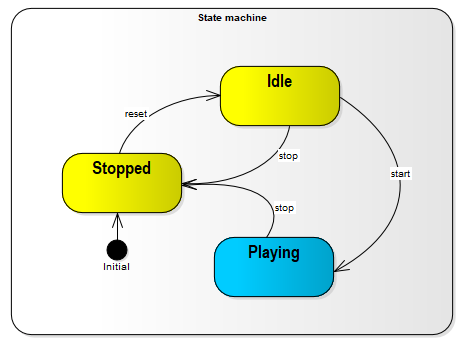
\includegraphics[width=0.8\linewidth]{/Users/Makki/Documents/candy-grabber/StateMachine.png}
\caption{\ac{UML} Diagramm der Klasse Achse}\label{fig:uml_state}
\end{figure}
%
\subsection{Softwarekomponenten und Libraries}
Verwendete Libraries und Node-RED Frameworks. Genaue Beschreibung der Klassen des Candy Grabbers.
%
\subsection{HMI Entwurf}
Benötigte Taster, Schalter, Informationen und Layout
%--------------------------------------------------------------UMSETZUNG
%\chapter{Umsetzung}
\section{Implementierung}
Zusammenführen der einzelnen Komponenten, Modifizierung der vorhandenen Hardware sowie Montage und Verbindung der Hardwaremodule. Erstellung der Programmierung. Während der Implementierung der Software wurde der Entwurf evaluiert und iterativ überarbeitet. Diese Änderungen wurden wiederum in die UML Diagramme übernommen um immer ein aktuelles Bild vom Stand des Systems zu erhalten. Die unterschiedlichen Versionen der UML Diagramme wurden ebenso wie die Versionen der Software in einem GIT Repository abgelegt.
%
\subsection{Modifizierung der Hardware und Montage}
%\begin{figure}[H]%
%        		\begin{minipage}[t]{\linewidth}%
%          	%\begin{center}%
%			\begin{minipage}{0.5\linewidth}
%				\begin{center}%
%           				\includegraphics[width=0.9\linewidth]{./PICs/verkabelung_motoren_vorher.png}%
%				\end{center}%
%			\end{minipage}
%			\begin{minipage}{0.5\linewidth}
%				\begin{center}
%           				\includegraphics[width=0.9\linewidth]{./PICs/verkabelung_motoren_nachher.png}%
%				\end{center}%
%			\end{minipage}
%			\caption{Verkabelung der Grenztaster und Motoren der x- und y-Achse vor und nach den vorgenommenen Modifizierungen}%
%			\label{fig:HWmodified}%
%          	%\end{center}%
%        		\end{minipage}%PackMLsimple copy
%\end{figure}%
%
\subsection{Programmierung}
Node-RED Flow Erstellung sowie Implementierung eigener Nodes in Java Script.
Erstellung der Klassen, Hardware Abstraktion und Erstellung des Python Programms für manuelle Bedienung. Repräsentation des Python Objekts im OPC UA Adressraum. Programmierung des Ablaufs für Remote Bedienung über Server und Node-RED Flow.
\subsection{Versionierung und Dokumentation}
Erstellung eines Git Repositories. Lesbarkeit des Codes und Einfügen von Kommentaren.
\subsection{Systemintegration und Tests}
Hardwareentwurf und Einbau aller Komponenten in den Candy Grabber. Beschriftung der Kabelverbindungen und Klemmen an der Hardware. Durchführung von Software-tests und Code-Hygiene (Debugging und Kommentare). Durchführung von Funktionstests.
%
\clearpage
\chapter{Ergebnisse}
Hier werden die Ergebnisse präsentiert. Ansichten der Umsetzung (Hardware, HMI).
\begin{table}[!htbp]
\caption{Umgesetzte Arbeitspakete}
\centering
\begin{tabular}{| p{0.33\linewidth}| p{0.33\linewidth} | p{0.33\linewidth}|}\hline
\rowcolor[gray]{0.8}Analyse und Planung & &\\\hline
Auswahl eines \ac{IOT} Geräts & Auswahl zusätzlich benötigter Hardware & Gründliche Dokumentation\\\hline
Analyse der Original Hardware & Erstellung Sensor/Aktor Liste \newline Entwurf Schaltplan & Anschluss an Rechner\\\hline
\rowcolor[gray]{0.8}Systementwurf &&\\\hline
Hardware Abstraktion und Schnittstellen & Systementwurf \newline Klassendiagramm erstellen & Ablauf planen \newline Ablaufdiagramm erstellen\\\hline
Schnittstellen und Systemgrenzen definieren & Methoden und Properties \newline definieren & Steuerungsprogramm erstellen\\\hline
\rowcolor[gray]{0.8}Systementwicklung &&\\\hline
Versuchsaufbauten erstellen & Auswahl der Toolchain &  Aufsetzen eines Servers \\\hline
Kommunikation mit Client & Webapplikation erstellen & Videostream einrichten\\\hline
\end{tabular}
\end{table}
%
\clearpage
\chapter{Zusammenfassung und Ausblick}
Evaluierung der Ergebnisse durch Vergleich mit den Anforderungen. Was wurde nicht implementiert und warum. Was sind die nächsten Schritte, wie könnte das System noch verbessert werden.
% Hier beginnen die Verzeichnisse.
%

%----------------------------------ZIELE
%\section{Projektziele}
%Recherche zu \ac{IOT} und Rapid-Prototyping im \ac{IOT} Bereich. Erstellen einer Übersicht von Tools die speziell für Prototyping entwickelt wurden. Gegenüberstellung und Diskussion der Vor- und Nachteile der vorgestellten Modelle und Methoden für die Anwendung in dieser Arbeit. Recherche über:
%\begin{itemize}
%	\item \ac{IOT} Architektur, Schichtmodelle
%	%\item Schnittstellen
%	\item Protokolle
%	\item Softwareplattformen
%	\item \ac{IOT} Geräte (\ac{IOT} devices)
%\end{itemize}
%Auswahl der Toolchain und Erstellen der \ac{IOT} Applikation für den Candy Grabber:
%\begin{itemize}
%	\item Hardware Auswahl
%	\item Hardware über GPIOs steuerbar, Motoren über Motorsteuerung (H-Brücken / Motor-Modul) steuerbar.
%	\item Umsetzung der Transportschicht, Versenden/Austauschen von Datenpaketen.
%	\item Erstellung einer Anwendung und Bereitstellung im Internet (Webdienst bereitstellen)
%\end{itemize}
%Bewertung der Umsetzung nach folgenden Qualitätskriterien:
%\begin{itemize}
%	\item Simplizität
%	\item Kosten
%	\item Skalierbarkeit
%	%\item Energieverbrauch
%	\item Modularität
%	\item Nachvollziehbarkeit
%\end{itemize}
%----------------------------------------------------ZUSAMMENFASSUNG

%\rowcolor[gray]{0.8}Systemintegration &&\\\hline
%\section{Meilensteine}
%{\color{red}Zum Zwecke der Messbarkeit, hier noch eine zeitliche Einteilung als Richtlinie zur Umsetzung des Projekts:}
%%Tabelle Meilensteine
\begin{table}[!htbp]
\caption{Diese Tabelle dient zur Überprüfung des Projektfortschritts und ist kein Bestandteil der schriftlichen Arbeit}
\centering
\begin{tabular}{| p{0.8\linewidth}| p{0.2\linewidth} |}\hline
Meilensteine & Zeitplan\\\hline
Aufsetzen des IoT Device (Raspberry Pi) &\cellcolor{green} Anfang März\\
Formulieren der Ziele & \cellcolor{green} 08.März\\
(zusätzliche) Hardware Auswahl und Abgabe Bestellliste &\cellcolor{green} 16.März\\
Hardware steuerbar über Rechner & \cellcolor{yellow} 30.März\\
Recherche zum Stand der Technik & \cellcolor{yellow} 14.April\\
Auswahl und Installation der Toolchain & \cellcolor{green} 30.April\\
Implementierung der IoT Anwendung & \cellcolor{green} 30.Mai\\
Präsentation des Candy Grabbers, Erstellung eines Videos & 13.Juni\\
Bewertung der Umsetzung und Fertigstellung der BA Arbeit & 16.Juni\\\hline
\end{tabular}
\end{table}
\clearpage
\ifthenelse{\equal{\FHTWCitationType}{HARVARD}}{}{\bibliographystyle{gerabbrv}}
\bibliography{Literatur}
\clearpage

% Das Abbildungsverzeichnis
\listoffigures
\clearpage

% Das Tabellenverzeichnis
\listoftables
\clearpage

% Das Quellcodeverzeichnis
\listofcode
\clearpage

\phantomsection
\addcontentsline{toc}{chapter}{\listacroname}
\chapter*{\listacroname}
\begin{acronym}[XXXXX]
	\acro{API}[API]{Application Programming Interface}
	\acro{BMK}[BMK]{Betriebsmittelkennzeichen}
	\acro{CIOT}[CIoT]{Commercial Internet of Things}
	\acro{CoAP}[CoAP]{Constrained Application Protocol}
	\acro{CSI}[CSI]{Camera Serial Interface}
	\acro{ETSI}[ETSI]{European Telecommunications Standards Institute}
	\acro{GPIO}[GPIO]{General Purpose Input/Output}
	\acro{GUID}[GUID]{Globally Unique Identifier}
	\acro{HMI}[HMI]{Human Machine Interface}
	\acro{HTTP}[HTTP]{Hypertext Transfer Protocol}
	\acro{IETF}{IETF}{Internet Engineering Task Force}
	\acro{IEEE}[IEEE]{Institute of Electrical and Electronics Engineers}
	\acro{I2C}[I2C]{Inter-Integrated Circuit}
	\acro{IIOT}[IIoT]{Industrial Internet of Things}
	\acro{IOT}[IoT]{Internet of Things}
	\acro{JPEG}[JPEG]{Joint Photographic Experts Group}
	\acro{LAN}[LAN]{Local Area Network}
	\acro{MJPEG}[MJPEG]{Motion JPEG}
	\acro{MPEG}[MPEG]{Moving Picture Experts Group}
   	\acro{MQTT}[MQTT]{Message Queuing Telemetry Transport}
	\acro{OPC UA}[OPC UA]{OPC Unified Architecture}
   	\acro{OSI}[OSI]{Open Systems Interconnection}
	\acro{PWM}[PWM]{Pulsweitenmodulation}
	\acro{REST}[REST]{Representational State Transfer}
	\acro{RTSP}[RTSP]{Real-Time Streaming Protocol}
	\acro{SBC}[SBC]{Single board computer}
   	\acro{SOA}[SOA]{Service-Oriented Architecture}
	\acro{SOAP}[SOAP]{Simple Object Access Protocol}
   	\acro{TCP}[TCP/IP]{Transmission Control Protocol/Internet Protocol}
	\acro{UDP}[UDP]{User Datagram Protocol}
	\acro{UML}[UML]{Unified Modeling Language}
	\acro{URI}[URI]{Uniform Resource Identifier}
	\acro{URL}[URL]{Uniform Resource Locator}
	\acro{W3C}[W3C]{World Wide Web Consortium}
   	\acro{WWW}[WWW]{World Wide Web}
   	\acro{WSN}[WSN]{Wired Sensor Network}
	\acro{XML}[XML]{Extensible Markup Language}
\end{acronym}

%
% Hier beginnt der Anhang.
%
\appendix
\chapter{UML Klassendiagramm des Candy Grabbers}
\begin{figure}[H]
\centering
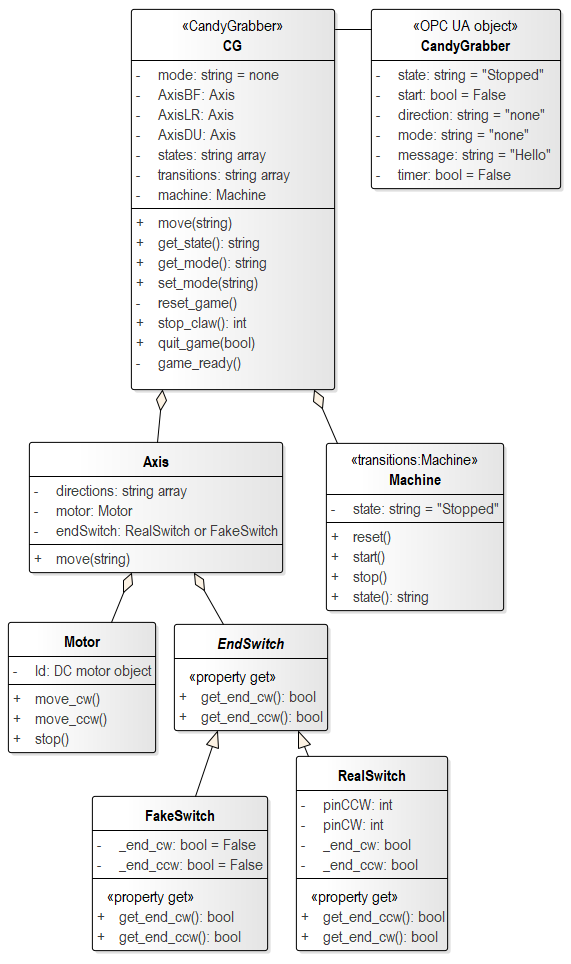
\includegraphics[width=0.9\linewidth]{/Users/Makki/Documents/candy-grabber/ClassDiagram_CG.png}
\caption{UML Klassendiagramm des \emph{CandyGrabber} Objekts}\label{fig:uml_class}
\end{figure}
%
\chapter{Node-RED Flow}
\begin{figure}[H]
\centering
\includegraphics[width=1.3\linewidth, angle=270]{./PICs/nodered_flow_cg.png}
\caption{Node-RED Flow des Candy Grabbers}\label{fig:nodered_flow}
\end{figure}
%
\chapter{Quellcode Klasse Axis}
 \lstinputlisting
    [caption={Klasse Achse}
       \label{lst:axis},
       captionpos=t,language=Python]
 {/Users/Makki/Documents/candy-grabber/axis.py}
%
\chapter{Quellcode Klasse Candy Grabber}
 \lstinputlisting
    [caption={Candy Grabber Klasse und Zustandsautomat}
       \label{lst:stateMachine},
       captionpos=t,language=Python]
 {/Users/Makki/Documents/candy-grabber/stateMachine.py}
%
\clearpage
\chapter{Quellcode Programmcode}
 \lstinputlisting
    [caption={Programmcode des Candy Grabbers}
       \label{lst:candy_server},
       captionpos=t,language=Python]
 {/Users/Makki/Documents/candy-grabber/candy_server.py}
\end{document}

%\noindent Querverweise werden in \LaTeX{} automatisch erzeugt und verwaltet, damit sie leicht aktualisiert werden können. Hier wird zum Beispiel auf Abbildung \ref{Abb1} verwiesen.
%
%\begin{figure}[!htbp]
%\centering
%\includegraphics[width=0.5\linewidth]{PICs/buchruecken}
%\caption{Beispiel für die Beschriftung eines Buchrückens.}\label{Abb1}
%\end{figure}
%\begin{figure}[!htbp]
%\centering
%\includegraphics[width=0.5\linewidth]{PICs/buchruecken}
%\caption{2. Beispiel für die Beschriftung eines Buchrückens.}\label{Abb2}
%\end{figure}
%
%Und hier ist ein Verweis auf Tabelle \ref{tab1}. Das gezeigte Tabellenformat ist nur ein Beispiel. Tabellen können individuell gestaltet werden.
%
%\begin{table}[!htbp]
%\centering
%\caption{Semesterplan der Lehrveranstaltung \glqq Angewandte Mathematik\grqq.}\label{tab1}
%\begin{tabular}{| p{0.3\linewidth} | p{0.3\linewidth} | p{0.3\linewidth} |}\hline
%Datum & Thema & Raum\\\hline
%20.08.2008 & Graphentheorie & HS 3.13\\
%01.10.2008 & Biomathematik & HS 1.05\\\hline
%\end{tabular}
%\end{table}
%\begin{table}[!htbp]
%\centering
%\caption{2. Semesterplan der Lehrveranstaltung \glqq Angewandte Mathematik\grqq.}\label{tab2}
%\begin{tabular}{| p{0.3\linewidth} | p{0.3\linewidth} | p{0.3\linewidth} |}\hline
%Datum & Thema & Raum\\\hline
%20.08.2008 & Graphentheorie & HS 3.13\\
%01.10.2008 & Biomathematik & HS 1.05\\\hline
%\end{tabular}
%\end{table}
%
%Hier wird auf die Formel \ref{Gl1} verwiesen.
%
%\begin{align}
%x = -\frac{p}{2}\pm\sqrt{\frac{p^2}{4}-q}\label{Gl1}
%\end{align}
%\begin{align}
%x = -\frac{p}{2}\pm\sqrt{\frac{p^2}{4}-q}\label{Gl2}
%\end{align}
%
%\begin{lstlisting}[language=C++,name={1. Beispiel},label={sc:bsp:1}]
%#include <iostream>
%
%void SayHello(void)
%{
%    // Kommentar
%    cout << "Hello World!" << endl;
%}
%
%int main(int argc, char **argv)
%{
%    SayHello();
%    return 0;
%}
%\end{lstlisting}
%
%Literaturverweise sollten automatisch verwaltet werden, vor allem, wenn es viele Quellenverweise gibt. Beispiele sind  \cite{Ko05a}, \cite{Ko05b}, \cite{MiGo05}, \cite{TeGo14}, \cite{HuHa07}, \cite{HuZi10}, \cite{ZiKu07}, \cite{He07}, \cite{SIE11}, \cite{SIE14}, \cite{ISO98}, \cite{ATM11}, \cite{Hu11}, \cite{Po10}. Das verwendete Zitierformat (bzw.~das Format des Literaturverzeichnisses) ist entspechend der Vorgaben der Studiengänge zu wählen.
%Es wird dringend empfohlen, BibTeX~zu verwenden (wie in diesem Beispiel).
%
%\chapter{Dritte Überschrift der Tiefe 1 (chapter)}
%\begin{figure}[!htbp]
%\centering
%\includegraphics[width=0.5\linewidth]{PICs/buchruecken}
%\caption{3. Beispiel für die Beschriftung eines Buchrückens.}\label{Abb3}
%\end{figure}
%\begin{figure}[!htbp]
%\centering
%\includegraphics[width=0.5\linewidth]{PICs/buchruecken}
%\caption{4. Beispiel für die Beschriftung eines Buchrückens.}\label{Abb4}
%\end{figure}
%
%
%\begin{table}[!htbp]
%\centering
%\caption{3. Semesterplan der Lehrveranstaltung \glqq Angewandte Mathematik\grqq.}\label{tab3}
%\begin{tabular}{| p{0.3\linewidth} | p{0.3\linewidth} | p{0.3\linewidth} |}\hline
%Datum & Thema & Raum\\\hline
%20.08.2008 & Graphentheorie & HS 3.13\\
%01.10.2008 & Biomathematik & HS 1.05\\\hline
%\end{tabular}
%\end{table}
%\begin{table}[!htbp]
%\centering
%\caption{4. Semesterplan der Lehrveranstaltung \glqq Angewandte Mathematik\grqq.}\label{tab4}
%\begin{tabular}{| p{0.3\linewidth} | p{0.3\linewidth} | p{0.3\linewidth} |}\hline
%Datum & Thema & Raum\\\hline
%20.08.2008 & Graphentheorie & HS 3.13\\
%01.10.2008 & Biomathematik & HS 1.05\\\hline
%\end{tabular}
%\end{table}
%
%\begin{align}
%x = -\frac{p}{2}\pm\sqrt{\frac{p^2}{4}-q}\label{Gl3}
%\end{align}
%\begin{align}
%x = -\frac{p}{2}\pm\sqrt{\frac{p^2}{4}-q}\label{Gl4}
%\end{align}
%\begin{lstlisting}[language=C++,name={2. Beispiel},label={sc:bsp:2}]
%#include <iostream>
%
%void SayHello(void)
%{
%    // Kommentar
%    cout << "Hello World!" << endl;
%}
%
%int main(int argc, char **argv)
%{
%    SayHello();
%    return 0;
%}
%\end{lstlisting}
